\chapter{Summarizing Data}
\label{summarizingData}

After collecting data, the next stage in the investigative process is to summarize the data. Graphical displays allow us to visualize and better understand the important features of a data set.

\section{Examining numerical data}
\label{numericalData}
In this section we will focus on numerical variables. The \data{email50} and \data{county} data sets from Section~\ref{dataBasics} provide rich opportunities for examples. Recall that outcomes of numerical variables are numbers on which it is reasonable to perform basic arithmetic operations. For example, the \var{pop2010} variable, which represents the populations of counties in 2010, is numerical since we can sensibly discuss the difference or ratio of the populations in two counties. On the other hand, area codes and zip codes are not numerical, but rather they are~categorical variables.


\subsection{Scatterplots for paired data}
\label{scatterPlots}

\index{data!email50|(}

Sometimes researchers wish to see the relationship between two variables. When we talk of a relationship or an association between variables, we are interested in how one variable behaves as the other variable increases or decreases.

A \term{scatterplot} provides a case-by-case view of data that illustrates the relationship between two numerical variables. In Figure~\vref{county_fed_spendVsPoverty}, a scatterplot was used to examine how federal spending and poverty were related in the \data{county} data set. Another scatterplot is shown in Figure~\ref{email50LinesCharacters}, comparing the number of line breaks (\var{line\_\hspace{0.3mm}breaks}) and number of characters (\var{num\_\hspace{0.3mm}char}) in emails for the \data{email50} data set. In any scatterplot, each point represents a single case. Since there are 50 cases in \data{email50}, there are 50 points in Figure~\ref{email50LinesCharacters}.

\textPE{\setlength{\captionwidth}{0.885\textwidth}}

\begin{figure}[h]
   \centering
   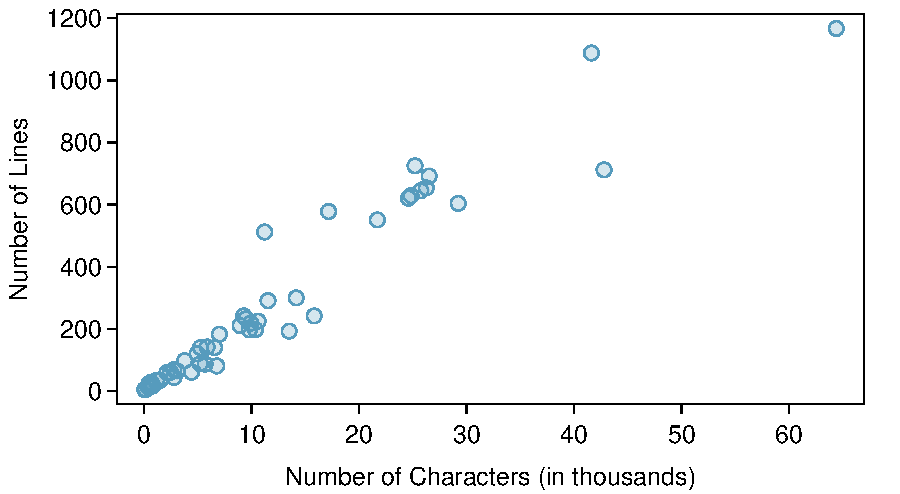
\includegraphics[width=0.75\textwidth]{ch_summarizing_data/figures/email50LinesCharacters/email50LinesCharacters}
   \caption{A scatterplot of \var{line\_\hspace{0.3mm}breaks} versus \var{num\_\hspace{0.3mm}char} for the \data{email50} data.}
   \label{email50LinesCharacters}
\end{figure}

\textPE{\setlength{\captionwidth}{\mycaptionwidth}}

\begin{example}{A scatterplot requires paired data. What does \term{paired data} mean?}
We say observations are \emph{paired} when the two observations correspond to each other. In unpaired data, there is no such correspondence. Here the two observations correspond to a particular email.
\end{example}

The variable that is suspected to be the response variable is plotted on the vertical (y)~axis and the variable that is suspected to be the explanatory variable is plotted on the horizontal (x)~axis. In this example, the variables could be switched since either variable could reasonably serve as the explanatory variable or the response variable.

\Comment{Adjusted wording in tip box below, but kept themes.}

\begin{tipBox}{\tipBoxTitle{Drawing scatterplots}
(1)~Decide which variable should go on each axis. Draw and label the two axes. \\
(2)~Note the range of each variable, and add tick marks and scales to each~axis. \\
(3)~Plot the dots as you would on an (\textit{x}, \textit{y}) coordinate plane.}
\end{tipBox}

The association between two variables can be \termsub{positive}{positive association} or \termsub{negative}{negative association}, or there can be no association. Positive association means that larger values of the first variable are associated with larger values of the second variable. Additionally, the association can follow a linear trend or a curved (nonlinear) trend.

\begin{exercise}What would it mean for two variables to have a \emph{negative} association? What about \emph{no} association?\footnote{Negative association implies that larger values of the first variable are associated with smaller values of the second variable. No association implies that the values of the second variable tend to be independent of changes in the first variable.}
\end{exercise}

\begin{exercise}
What does the scatterplot in Figure~\ref{email50LinesCharacters} reveal about the email data?\footnote{The association between the number of characters in an email and the number of lines in an email is positive (when one is larger, the other tends to be larger as well). As the number of characters increases, number of lines increases is an approximately linear fashion.}
\end{exercise}

\index{data!cars|(}
\begin{example}{Consider a new data set of 54 cars with two variables: vehicle price and~weight.\footnote{Subset of data from \urlwofont{http://www.amstat.org/publications/jse/v1n1/datasets.lock.html}} A scatterplot of vehicle price versus weight is shown in Figure~\ref{carsPriceVsWeight}. What can be said about the relationship between these variables?}
The relationship is evidently nonlinear, as highlighted by the dashed line. This is different from previous scatterplots we've seen, such as Figure~\vref{county_fed_spendVsPoverty} and Figure~\ref{email50LinesCharacters}, which show relationships that are very linear.

\begin{figure}[h]
   \centering
   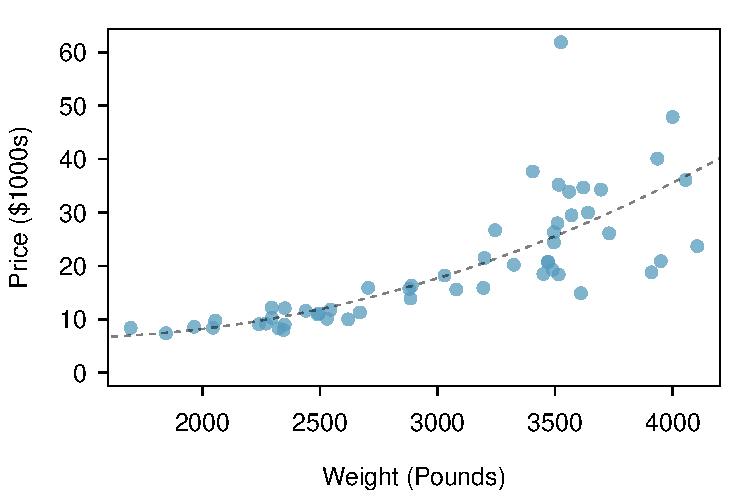
\includegraphics[width=0.65\textwidth]{ch_summarizing_data/figures/carsPriceVsWeight/carsPriceVsWeight}
   \caption{A scatterplot of \var{price} versus \var{weight} for 54 cars.}
   \label{carsPriceVsWeight}
\end{figure}
\end{example}
\index{data!cars|)}

\begin{exercise}
\Comment{Adjusted solution.} Describe two variables that would have a horseshoe shaped (i.e. ``U"-shaped) association in a scatterplot.\footnote{Consider a variable that represents something that is only good in moderation. Water consumption fits this description since water becomes toxic when consumed in excessive quantities. If health was represented on the vertical axis and water consumption on the horizontal axis, then we would create an upside down ``U''~shape.}
\end{exercise}


\subsection{Stem-and-leaf plots and dot plots}
\label{dotPlot}

Sometimes two variables is one too many: only one variable may be of interest. In these cases we want to focus not on the association between two variables, but on the distribution of a single variable. The term \term{distribution} refers to the values that a variable takes and the frequency of these values. Let's take a closer look at the \data{email50} data set and focus on the number of characters in each email. To simplify the data, we will round the numbers and record the values in thousands. Thus, 22105 is recorded as 22.

\textPE{\setlength{\captionwidth}{0.9\textwidth}}

\begin{table}[ht]
\centering
\begin{tabular}{rrrrrrrrrr}
  \hline
 22 & 0 & 64 & 10 & 6 & 26 & 25 & 11 & 4 & 14 \\
  7 & 1 & 10 & 2 & 7 & 5 & 7 & 4 & 14 & 3 \\
   1 & 5 & 43 & 0 & 0 & 3 & 25 & 1 & 9 & 1 \\
  2 & 9 & 0 & 5 & 3 & 6 & 26 & 11 & 25 & 9 \\
  42 & 17 & 29 & 12 & 27 & 10 & 0 & 0 & 1 & 16 \\
   \hline
\end{tabular}
\caption{The number of characters, in thousands, for the data set of 50~emails.}
\end{table}

\textPE{\setlength{\captionwidth}{\mycaptionwidth}}

Rather than look at the data as a list of numbers, which makes the distribution difficult to discern, we will organize it into a table called a \term{stem-and-leaf plot} shown in Figure~\ref{stemandleafemail50}. In a stem-and-leaf plot, each number is broken into two parts. The first part is called the \term{stem} and consists of the beginning digit(s). The second part is called the \term{leaf} and consists of the final digits(s). The stems are written in a column in ascending order, and the leaves that match up with those stems are written on the corresponding row. Figure~\ref{stemandleafemail50} shows a stem-and-leaf plot of the number of characters in 50 emails. The stem represents the ten thousands place and the leaf represents the thousands place. For example, \texttt{1 $|$ 2} corresponds to 12 thousand. When making a stem-and-leaf plot, remember to include a legend that describes what the stem and what the leaf represent. Without this, there is no way of knowing if 1 $|$ 2  represents 1.2, 12, 120, 1200, etc.

\begin{figure}[h]
\begin{verbatim}
                   0 | 00000011111223334455566777999
                   1 | 0001124467
                   2 | 25556679
                   3 |
                   4 | 23
                   5 |
                   6 | 4

                 Legend: 1 | 2 = 12,000
\end{verbatim}
\caption{A stem-and-leaf plot of the number of characters in 50 emails.}
\label{stemandleafemail50}
\end{figure}

\begin{exercise}There are a lot of numbers on the first row of the stem-and-leaf plot. Why is this the case?\footnote{There are a lot of numbers on the first row because there are a lot of values in the data set less than 10 thousand.}
\end{exercise}

When there are too many numbers on one row or there are only a few stems, we \emph{split} each row into two halves, with the leaves from 0-4 on the first half and the leaves from 5-9 on the second half. The resulting graph is called a \termsub{split stem-and-leaf plot}{stem-and-leaf plot!split stem-and-leaf plot}. Figure~\ref{splitstemandleaf50email} shows the previous stem-and-leaf redone as a split stem-and-leaf.

\begin{figure}[h]
\begin{verbatim}
                          0 | 000000111112233344
                          0 | 55566777999
                          1 | 00011244
                          1 | 67
                          2 | 2
                          2 | 5556679
                          3 |
                          3 |
                          4 | 23
                          4 |
                          5 |
                          5 |
                          6 | 4

                        Legend: 1 | 2 = 12,000
\end{verbatim}
\caption{A split stem-and-leaf.}
\label{splitstemandleaf50email}
\end{figure}

\begin{exercise}
What is the smallest number in this data set? What is the largest?\footnote{The smallest number is less than 1 thousand, and the largest is 64 thousand. That is a big range!}
\end{exercise}

%\Add{Many emails are short, but some are very long. An investigation of the data would reveal that most of the long emails use the HTML format, which means most of the characters in those emails are used to format the email rather than provide text.} % Omitting since it doesn't have any clear connection to the surrounding text.

Another simple graph for numerical data is a dot plot. A~\term{dot plot} uses dots to show the \term{frequency}, or number of occurrences, of the values in a data set. The higher the stack of dots, the greater the number occurrences there are of the corresponding value. An example using the same data set, number of characters from 50 emails, is shown in Figure~\ref{emailCharactersDotPlotStacked}.

\begin{figure}[h]
   \centering
   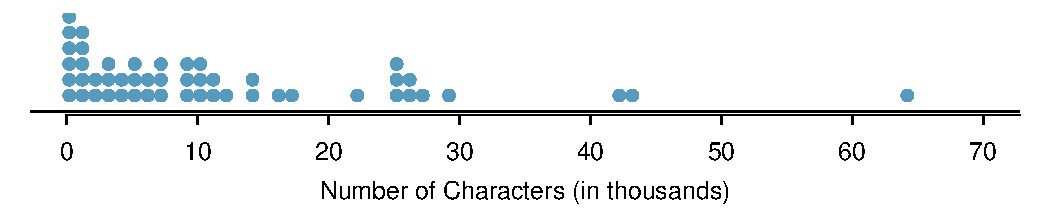
\includegraphics[width=0.9\textwidth]{ch_summarizing_data/figures/emailCharactersDotPlot/emailCharactersDotPlotStackedRounded}
   \caption{A dot plot of \var{num\_\hspace{0.3mm}char} for the \data{email50} data set.}
   \label{emailCharactersDotPlotStacked}
\end{figure}

\begin{exercise}
Imagine rotating the dot plot 90 degrees clockwise. What do you notice?\footnote{It has a similar shape as the stem-and-leaf plot! The values on the horizontal axis correspond to the stems and the number of dots in each interval correspond the number of leaves needed for each stem.}
\end{exercise}

These graphs make it easy to observe important features of the data, such as the location of clusters and presence of gaps.

\begin{example}{Based on both the stem-and-leaf and dot plot, where are the values clustered and where are the gaps for the \data{email50} data set?}
There is a large cluster in the 0 to less than 20 thousand range, with a peak around 1 thousand. There are gaps between 30 and 40 thousand and between the two values in the 40 thousands and the largest value of approximately 64 thousand.
\end{example}

Additionally, we can easily identify any observations that appear to be unusually distant from the rest of the data. Unusually distant observations are called \termsub{outliers}{outlier}. Later in this chapter we will provide numerical rules of thumb for identifying outliers. For now, it is sufficient to identify them by observing gaps in the graph. In this case, it would be reasonable to classify the emails with character counts of 42 thousand, 43 thousand, and 64 thousand as outliers since they are numerically distant from most of the data.


\begin{termBox}{\tBoxTitle{Outliers are extreme}
An \term{outlier} is an observation that appears extreme relative to the rest of the data.}
\end{termBox}


\begin{tipBox}{\tipBoxTitle{Why it is important to look for outliers}
Examination of data for possible outliers serves many useful purposes, including\vspace{-2mm}
\begin{enumerate}
\setlength{\itemsep}{0mm}
\item Identifying asymmetry in the distribution.
\item Identifying data collection or entry errors. For instance, we re-examined the email purported to have 64 thousand characters to ensure this value was accurate.
\item Providing insight into interesting properties of the data.\vspace{0.5mm}
\end{enumerate}}
\end{tipBox}

\begin{exercise}
The observation 64 thousand, a suspected outlier, was found to be an accurate observation. What would such an observation suggest about the nature of character counts in emails?\footnote{That occasionally there may be very long emails.}\end{exercise}

\begin{exercise}
Consider a data set that consists of the following numbers:  12, 12, 12, 12, 12, 13, 13, 14, 14, 15, 19. Which graph would better illustrate the data: a stem-and-leaf plot or a dot plot? Explain.\footnote{Because all the values begin with 1, there would be only one stem (or two in a split stem-and-leaf). This would not provide a good sense of the distribution. For example, the gap between 15 and 19 would not be visually apparent. A dot plot would be better here.}
\end{exercise}


\Comment{Separating Shape into a separate subsection than Histograms, since shape can be inferred from dot plot and stem-and-leaf as well}

\subsection{Histograms}
\label{histogramsAndShape}

Stem-and-leaf plots and dot plots are ideal for displaying data from small samples because they show the exact values of the observations and how frequently they occur. However, they are impractical for larger samples. \Add{For larger samples, }rather than showing the frequency of every value, we prefer to think of the value as belonging to a \emph{bin}. For example, in the \data{email50} data set, we create a table of counts for the number of cases with character counts between 0 and 5,000, then the number of cases between 5,000 and 10,000, and so on. Such a table, shown in Table~\ref{binnedNumCharTable}, is called a \term{frequency table}. Observations that fall on the boundary of a bin (e.g.~5,000) are \Add{generally} allocated to the lower bin.\footnote{This is called \emph{left inclusive}.} These binned counts are plotted as bars in Figure~\ref{email50NumCharHist} into what is called a \term{histogram} or \term{frequency histogram}, which resembles the stacked dot plot shown in Figure~\ref{emailCharactersDotPlotStacked}.

\begin{table}[ht]
\centering\small
\begin{tabular}{l ccc ccc ccc c}
  \hline
Characters & \\
(in thousands) & \raisebox{1.5ex}[0pt]{0-5} & \raisebox{1.5ex}[0pt]{5-10} & \raisebox{1.5ex}[0pt]{10-15} & \raisebox{1.5ex}[0pt]{15-20} & \raisebox{1.5ex}[0pt]{20-25} & \raisebox{1.5ex}[0pt]{25-30} & \raisebox{1.5ex}[0pt]{$\cdots$} & \raisebox{1.5ex}[0pt]{55-60} & \raisebox{1.5ex}[0pt]{60-65} \\
  \hline
Count & 19 & 12 & 6 & 2 & 3 & 5 & $\cdots$ & 0 & 1 \\
  \hline
\end{tabular}
\caption{The counts for the binned \var{num\_\hspace{0.3mm}char} data.}
\label{binnedNumCharTable}
\end{table}

\begin{figure}[bth]
   \centering
   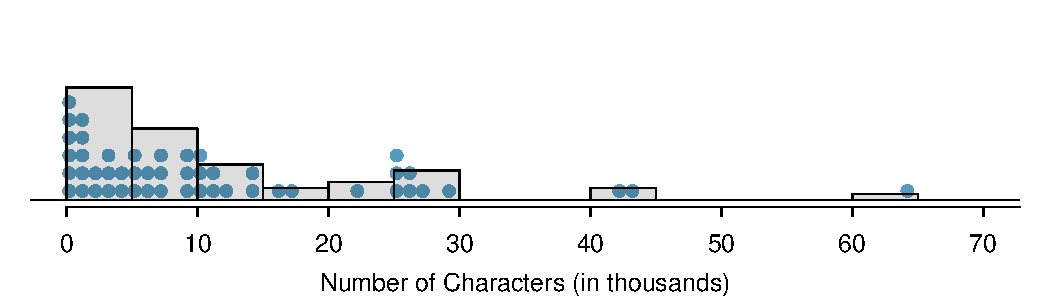
\includegraphics[width=0.82\textwidth]{ch_summarizing_data/figures/emailCharactersDotPlot/emailCharactersDotPlotStackedRoundedHist}
   \caption{A histogram of \var{num\_\hspace{0.3mm}char}. This histogram is drawn over the corresponding dot plot.}
   \label{emailCharactersDotPlotStackedRoundedHist}
\end{figure}

\begin{figure}[bth]
   \centering
   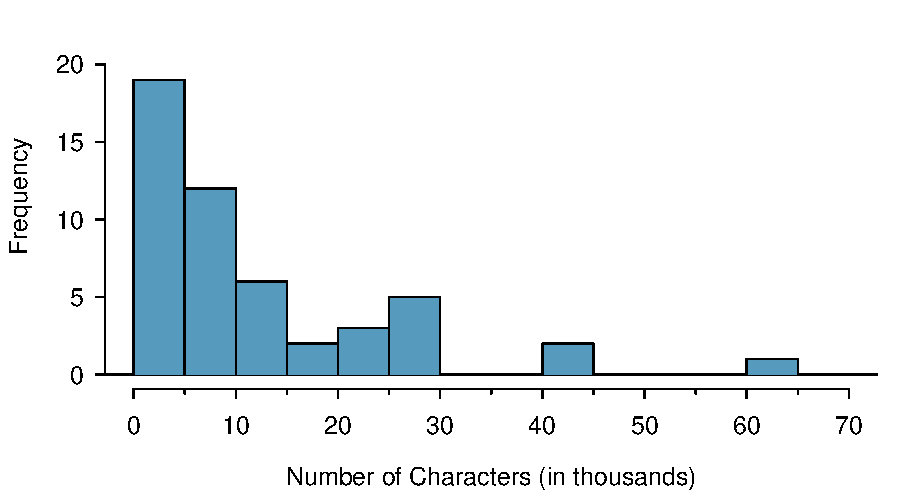
\includegraphics[width=0.82\textwidth]{ch_summarizing_data/figures/email50NumCharHist/email50NumCharHist}
   \caption{A histogram of \var{num\_\hspace{0.3mm}char}. This histogram uses bins or class intervals of width 5.}
   \label{email50NumCharHist}
\end{figure}

\begin{exercise}
What can you see in the dot plot and stem-and-leaf plot that you cannot see in the frequency histogram?\footnote{Character counts for individual emails.}
\end{exercise}

\begin{tipBox}{\tipBoxTitle{Drawing histograms}
1. The variable is always placed on the horizontal axis. Before drawing the histogram, label both axes and draw a scale for each. \\[2mm]
2. Draw bars such that the height of the bar is the frequency of that bin and the width of the bar corresponds to the bin width.}
\end{tipBox}

Histograms provide a view of the \term{data density}. Higher bars represent where the data are relatively more common. For instance, there are many more emails between 0 and 10,000 characters than emails between 10,000 and 20,000 in the data set. The bars make it easy to see how the density of the data changes relative to the number of characters.

\begin{example}{How many emails had fewer than 10 thousand characters?}The height of the bars corresponds to frequency. There were 19 cases from 0 to less than 5 thousand and 12 cases from 5 thousand to less than 10 thousand, so there were $19+12=31$ emails with fewer than 10 thousand characters.
\end{example}

\begin{example}{Approximately how many emails had fewer than 1 thousand chacters?} Based just on this histogram, we cannot know the exact answer to this question. We only know that 19 emails had between 0 and 5 thousand characters. If the number of emails is evenly distribution on this interval, then we can estimate that approximately 19/5~$\approx$ 4 emails fell in the range between 0 and 1 thousand.
\end{example}

\begin{example}{What \emph{percent} of the emails had 10 thousand or more characters?}
\Comment{I don't think the new sentence is adding clarity. It says we will first find the ``or more'' case, but then brings up the ``fewer than'' case. I had to read the surrounding text twice since I thought this new sentence's wording was a mistake.} \Add{First find the number of emails that had 10 thousand or more characters.} From the first example, we know that 31 emails had fewer than 10 thousand characters. Since there are 50 emails in total, there must be 19 emails that have 10 thousand or more characters. To find the percent, compute $19/50 = 0.38 = 38\%$.
\end{example}

Sometimes questions such as the ones above can be answered more easily with a \term{cumulative frequency histogram}. This type of histogram shows cumulative, or total, frequency achieved by each bin, rather than the frequency in that particular bin.

\begin{table}[ht]
\centering\small
\begin{tabular}{l ccc ccc ccc c}
  \hline
Characters & \\
(in thousands) & \raisebox{1.5ex}[0pt]{0-5} & \raisebox{1.5ex}[0pt]{5-10} & \raisebox{1.5ex}[0pt]{10-15} & \raisebox{1.5ex}[0pt]{15-20} & \raisebox{1.5ex}[0pt]{20-25} & \raisebox{1.5ex}[0pt]{25-30} &  \raisebox{1.5ex}[0pt]{30-35} &\raisebox{1.5ex}[0pt]{$\cdots$} & \raisebox{1.5ex}[0pt]{55-60} & \raisebox{1.5ex}[0pt]{60-65} \\
  \hline
Cumulative &\\
Frequency &  \raisebox{1.5ex}[0pt]{19} & \raisebox{1.5ex}[0pt]{31} & \raisebox{1.5ex}[0pt]{37} & \raisebox{1.5ex}[0pt]{39} & \raisebox{1.5ex}[0pt]{42} & \raisebox{1.5ex}[0pt]{47} & \raisebox{1.5ex}[0pt]{47} & \raisebox{1.5ex}[0pt]{$\cdots$} & \raisebox{1.5ex}[0pt]{49} & \raisebox{1.5ex}[0pt]{50} \\
  \hline
\end{tabular}
\caption{The cumulative frequencies for the binned \var{num\_\hspace{0.3mm}char} data.}
\label{binnedNumCharTableCumulative}
\end{table}

\begin{figure}[bth]
   \centering
   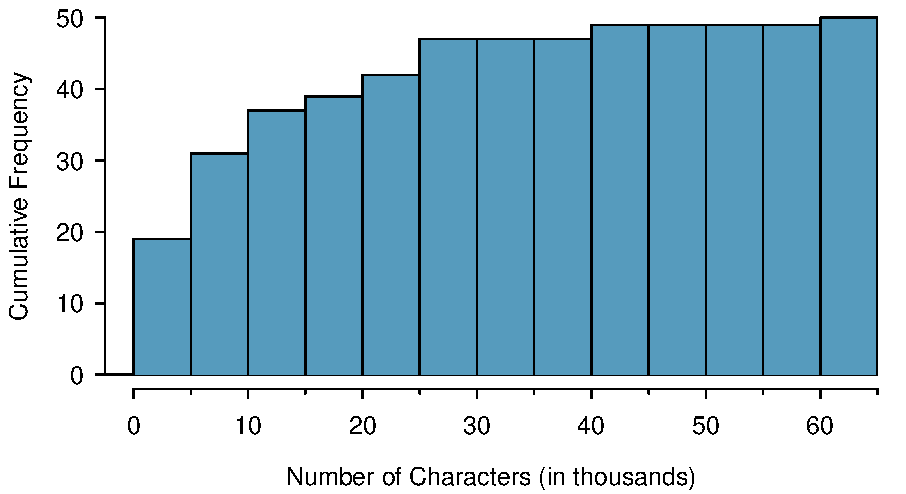
\includegraphics[width=0.82\textwidth]{ch_summarizing_data/figures/email50NumCharHist/email50NumCharCumulativeFreqHist}
   \caption{A cumulative frequency histogram of \var{num\_\hspace{0.3mm}char}. This histogram uses bins or class intervals of width 5.}
   \label{email50NumCharCumulativeFreqHist}
\end{figure}

\begin{example}{How many of the emails had fewer than 20 thousand characters?}
By tracing the height of the 15-20 thousand bin over to the vertical axis, we can see that it has a height just under 40 on the cumulative frequency scale. Therefore, we estimate that $\approx$39 of the emails had fewer than 30 thousand characters. Note that, unlike with a regular frequency histogram, we do not add up the height of the bars in a cumulative frequency histogram because each bar already represents a cumulative sum.
\end{example}

\begin{example}{Using the cumulative frequency histogram, how many of the emails had 10-15 thousand characters?}
To answer this question, we do a subtraction. $\approx$39 had fewer than 15-20 thousand emails and $\approx$37 had fewer than 10-15 thousand emails, so $\approx$2 must have had between 10-15 thousand emails.
\end{example}

\begin{example}{Approximately 25 of the emails had fewer than how many characters?}
This time we are given a cumulative frequency, so we start at 25 on the vertical axis and trace it across to see which bin it hits. It hits the 5-10 thousand bin, so 25 of the emails had fewer than a value somewhere between 5 and 10 thousand characters.
\end{example}

Knowing that 25 of the emails had fewer than a value between 5 and 10 thousand characters is useful information, but it is even more useful if we know what percent of the total 25 represents. Knowing that that there were 50 total emails tells us that $25 / 50 = 0.5 = 50\%$ of the emails had fewer than a value between 5 and 10 thousand characters. When we want to know what fraction or percent of the data meet a certain criteria, we use relative frequency instead of frequency. \termsub{Relative frequency}{relative frequency} is a fancy term for percent or proportion. It tells us how large a number is relative to the total.

Just as we constructed a frequency table, frequency histogram, and cumulative frequency histogram, we can construct a relative frequency table, relative frequency histogram, and cumulative relative frequency histogram.

\begin{exercise}
How will the \emph{shape} of the relative frequency histograms differ from the frequency histograms?\footnote{The shape will remain exactly the same. Changing from frequency to relative frequency involves dividing all the frequencies by the same number, so only the vertical scale (the numbers on the y-axis) change.}
\end{exercise}

\begin{caution}{Pay close attention to the vertical axis of a histogram}
{We can misinterpret a histogram if we forget to check whether the vertical axis represents frequency, relative frequency, cumulative frequency, or cumulative relative frequency.}
\end{caution}

%\Comment{insert relative frequency table and relative frequency histogram here?}

%\Comment{reference the relative frequency graph here since it is closer}


\subsection{Describing Shape}
\label{shape}

Frequency and relative frequency histograms are especially convenient for describing the \term{shape} of the data distribution\label{shapeFirstDiscussed}. Figure~\ref{email50NumCharHist} shows that most emails have a relatively small number of characters, while fewer emails have a very large number of characters. When data trail off to the right in this way and have a longer right \hiddenterm{tail}\index{skew!tail}, the shape is said to be \termsub{right skewed}{skew!right skewed}.\footnote{Other ways to describe data that are skewed to the right: \termni{skewed to the right}, \termni{skewed to the high end}, or \termni{skewed to the positive end}.}

Data sets with the reverse characteristic -- a long, thin tail to the left -- are said to be \termsub{left skewed}{skew!left skewed}. We also say that such a distribution has a long left tail. Data sets that show roughly equal trailing off in both directions are called \term{symmetric}.\index{skew!symmetric}

\begin{termBox}{\tBoxTitle{Long tails to identify skew}%
When data trail off in one direction, the distribution has a \term{long tail}. \index{skew!long tail|textbf} If a distribution has a long left tail, it is left skewed. If a distribution has a long right tail, it is right skewed.}
\end{termBox}

\begin{exercise}
Take a look at the dot plot in Figure~\ref{emailCharactersDotPlotStacked}. Can you see the skew in the data? Is it easier to see the skew in the frequency histogram, the dot plot, or the stem-and-leaf plot?\footnote{The skew is visible in all three plots. However, it is not easily visible in the cumulative frequency histogram.}
\end{exercise}

\begin{exercise}
\Comment{Adjusted the solution in the footnote.}
Would you expect the distribution of number of pets per household to be right skewed, left skewed, or approximately symmetric?  Explain.\footnote{We suspect most households would have 0, 1, or 2 pets but that a smaller number of households will have 3, 4, 5, or more pets, so there will be greater density over the small numbers, suggesting the distribution will have a long right tail and be right skewed.}
\end{exercise}

In addition to looking at whether a distribution is skewed or symmetric, histograms, stem-and-leaf plots, and dot plots can be used to identify modes. A \term{mode} is represented by a prominent peak in the distribution.\footnote{Another definition of mode, which is not typically used in statistics, is the value with the most occurrences. It is common to have \emph{no} observations with the same value in a data set, which makes this other definition useless for many real data sets.} There is only one prominent peak in the histogram of \var{num\_\hspace{0.3mm}char}.

Figure~\ref{singleBiMultiModalPlots} shows histograms that have one, two, or three prominent peaks. Such distributions are called \termsub{unimodal}{modality!unimodal}, \termsub{bimodal}{modality!bimodal}, and \termsub{multimodal}{modality!multimodal}, respectively. Any distribution with more than 2 prominent peaks is called multimodal. Notice that in Figure~\ref{email50NumCharHist} there was one prominent peak in the unimodal distribution with a second less prominent peak that was not counted since it only differs from its neighboring bins by a few observations.

\begin{figure}[h]
   \centering
   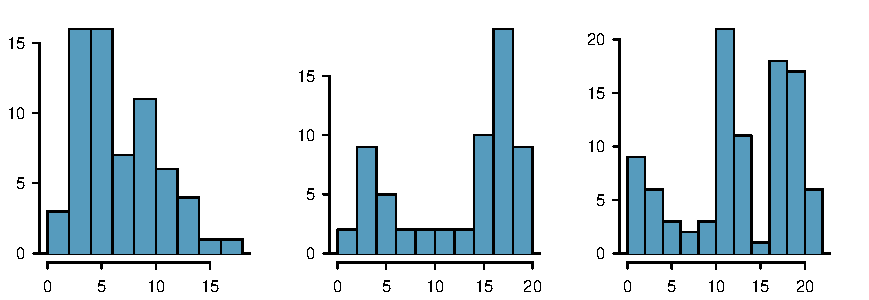
\includegraphics[width=\textwidth]{ch_summarizing_data/figures/singleBiMultiModalPlots/singleBiMultiModalPlots}
   \caption{Counting only prominent peaks, the distributions are (left to right) unimodal, bimodal, and multimodal.}
   \label{singleBiMultiModalPlots}
\end{figure}

\begin{exercise}
Height measurements of young students and adult teachers at a K-3 elementary school were taken. How many modes would you anticipate in this height data set?\footnote{There might be two height groups visible in the data set: one of the students and one of the adults. That is, the data are probably bimodal.}
\end{exercise}

\begin{tipBox}{\tipBoxTitle{Looking for modes}
Looking for modes isn't about finding a clear and correct answer about the number of modes in a distribution, which is why \emph{prominent} is not rigorously defined in this book. The important part of this examination is to better understand your data and how it might be structured.}
\end{tipBox}

%\Comment{maybe a separate section here on numerical summaries of (numerical) data}

\section{Numerical summaries and box plots}
\label{numericalSummariesAndBoxPlots}

\subsection{Measures of center}
\label{center}

In the previous section, we saw that modes can occur anywhere in a data set. Therefore, mode is not a measure of \term{center}. We understand the term \emph{center} intuitively, but quantifying what is the center can be a little more challenging. This is because there are different definitions of center. Here we will focus on the two most common: the mean and median.

The \term{mean}, sometimes called the \indexthis{average}{mean!average}, is a common way to measure the center of a distribution of data. To find the mean number of characters in the 50 emails, we add up all the character counts and divide by the number of emails. For computational convenience, the number of characters is listed in the thousands and rounded to the first decimal.
\begin{eqnarray}
\bar{x} = \frac{21.7 + 7.0 + \cdots + 15.8}{50} = 11.6
\label{sampleMeanEquation}
\end{eqnarray}
The sample mean is often labeled $\bar{x}$\marginpar[\raggedright$\bar{x}$\\\footnotesize sample\\ mean]{\raggedright$\bar{x}$\\\footnotesize sample\\ mean}. The letter $x$ is being used as a generic placeholder for the variable of interest, \var{num\_\hspace{0.3mm}char}, and the bar says it is the average number of characters in the 50 emails was 11,600.

\begin{termBox}{\tBoxTitle{Mean}
The sample mean of a numerical variable is computed as the sum of all of the observations divided by the number of observations:
\begin{eqnarray}
\bar{x} = \frac{1}{n}\sum{x_{i}} = \frac{x_1+x_2+\cdots+x_n}{n}
\label{meanEquation}
\end{eqnarray}
where $\sum$ is the capital Greek letter sigma and $\sum{x_{i}}$ means take the sum of all the individual $x$ values.
 $x_1, x_2, \dots, x_n$ represent the $n$ observed values.}
\end{termBox}

\begin{exercise}
Examine Equations~\eqref{sampleMeanEquation} and~\eqref{meanEquation} above. What does $x_1$ correspond to? And $x_2$? What does $x_i$ represent?\footnote{$x_1$ corresponds to the number of characters in the first email in the sample (21.7, in thousands), $x_2$ to the number of characters in the second email (7.0, in thousands), and $x_i$ corresponds to the number of characters in the $i^{th}$ email in the data set.}
\end{exercise}

\begin{exercise}
What was $n$ in this sample of emails?\footnote{The sample size was $n=50$.}
\end{exercise}

The \data{email50} data set represents a sample from a larger population of emails that were received in January and March. We could compute a mean for this population in the same way as the sample mean, however, the population mean has a special label: $\mu$\marginpar[\raggedright$\mu$\\\footnotesize population\\ mean]{\raggedright$\mu$\\\footnotesize population\\ mean}. \index{Greek!mu@mu ($\mu$)} The symbol $\mu$ is the Greek letter \emph{mu} and represents the average of all observations in the population. Sometimes a subscript, such as $_x$, is used to represent which variable the population mean refers to, e.g. $\mu_x$.

\begin{example}{The average number of characters across all emails can be estimated using the sample data. Based on the sample of 50 emails, what would be a reasonable estimate of $\mu_x$, the mean number of characters in all emails in the \data{email} data set? (Recall that \data{email50} is a sample from \data{email}.)}
The sample mean, 11,600, may provide a reasonable estimate of $\mu_x$. While this number will not be perfect, it provides a \emph{point estimate} of the population mean. In Chapter~\ref{foundationsForInference} and beyond, we will develop tools to characterize the reliability of point estimates, and we will find that point estimates based on larger samples tend to be more reliable than those based on smaller samples.
\end{example}

\begin{example}{We might like to compute the average income per person in the US. To do so, we might first think to take the mean of the per capita incomes across the 3,143 counties in the \data{county} data set. What would be a better approach?} \label{wtdMeanOfIncome}
The \data{county} data set is special in that each county actually represents many individual people. If we were to simply average across the \var{income} variable, we would be treating counties with 5,000 and 5,000,000 residents equally in the calculations. Instead, we should compute the total income for each county, add up all the counties' totals, and then divide by the number of people in all the counties. If we completed these steps with the \data{county} data, we would find that the per capita income for the US is \$27,348.43. Had we computed the \emph{simple} mean of per capita income across counties, the result would have been just \$22,504.70!
\end{example}

Example~\ref{wtdMeanOfIncome} used what is called a \term{weighted mean}\index{mean!weighted mean}, which will not be a key topic in this textbook. However, we have provided an online supplement on weighted means for interested readers:
\begin{center}
\urlwofont{http://www.openintro.org/stat/down/supp/wtdmean.pdf}
\end{center}

The median provides another measure of center. The \term{median} splits an ordered data set in half. There are 50 character counts in the \data{email50} data set (an even number) so the data are perfectly split into two groups of~25. We take the median in this case to be the average of the two middle observations: $(\text{6,768} + \text{7,012}) / 2 = \text{6,890}$. When there are an odd number of observations, there will be exactly one observation that splits the data into two halves, and in this case that observation is the median (no average needed).

\begin{termBox}{\tBoxTitle{Median: the number in the middle}
In an ordered data set, the \term{median} is the observation right in the middle. If there are an even number of observations, the median is the average of the two middle values.}
\end{termBox}

Graphically, we can think of the mean as the balancing point. The median is the value such that 50\% of the \emph{area} is to the left of it and 50\% of the \emph{area} is to the right of it.

%\Comment{insert histogram of email data set with mean and median indicated}.

\begin{figure}[h]
   \centering
   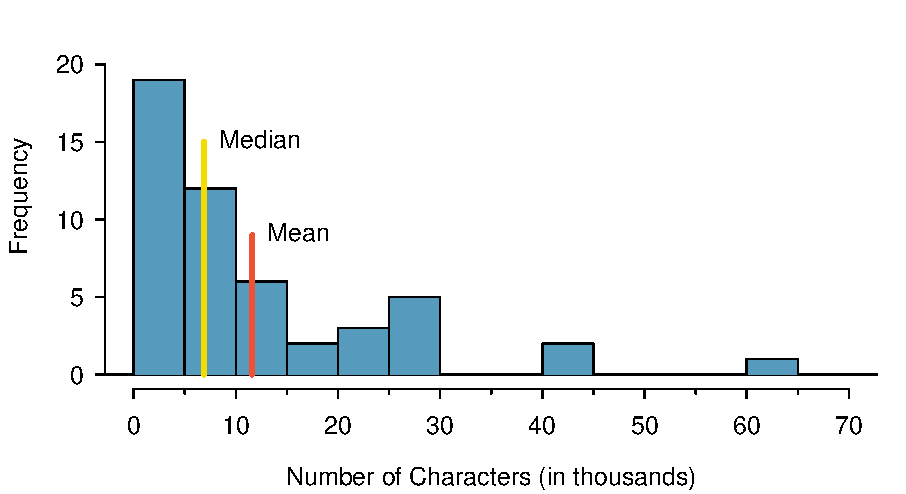
\includegraphics[width=0.8\textwidth]{ch_summarizing_data/figures/email50NumCharHist/email50NumCharHistWMeanMedian}
   \caption{A histogram of \var{num\_\hspace{0.3mm}char} with its mean and median shown.}
   \label{email50NumCharHistWMeanMedian}
\end{figure}

\begin{example}{Based on the data, why is the mean greater than the median in this data set?}
Consider the three largest values of 42 thousand, 43 thousand, and 64 thousand. These values drag up the mean because they substantially increase the sum (the~total). However, they do not drag up the median because their magnitude does not change the location of the middle value.
\end{example}

%\Comment{add box}.

\begin{termBox}{\tBoxTitle{The mean follows the tail}
In a right skewed distribution, the mean is greater than the median.

In a left skewed distribution, the mean is less than the median.

In a symmetric distribution, the mean and median are approximately equal.}
\end{termBox}

\begin{exercise}Consider the distribution of individual income in the United States. Which is greater: the mean or median? Why?\footnote{Because a small percent of individuals earn extremely large amounts of money while the majority earn a modest amount, the distribution is skewed to the right. Therefore, the mean is greater than the median.}
\end{exercise}

\subsection{Standard deviation as a measure of spread}
\label{variability}

The U.S. Census Bureau reported that in 2012, the median family income was \$62,241 and the mean family income was \$82,743.\footnote{\urlwofont{http://www.census.gov/hhes/www/income/}}

Is a family income of \$60,000 far from the mean or somewhat close to the mean? In order to answer this question, it is not enough to know the center of the data set and its \term{range} (maximum value - minimum value). We must know about the variability\index{variability} of the data set within that range. Low variability or small spread means that the values tend to be more clustered together. High variability or large spread means that the values tend to be far apart.

\begin{example}{Is it possible for two data sets to have the same range but different spread? If so, give an example. If not, explain why not.}
Yes. An example is:  {1, 1, 1, 1, 1, 9, 9, 9, 9, 9} and {1, 5, 5, 5, 5, 5, 5, 5, 5, 5, 9}.

The first data set has a larger spread because values tend to be farther away from each other while in the second data set values are clustered together at the mean.
\end{example}

Here, we introduce the standard deviation as a measure of spread. Though its formula is a bit tedious to calculate by hand, the standard deviation is very useful in data analysis and roughly describes how far away, on average, the observations are from the mean.

We call the distance of an observation from its mean its \term{deviation}. Below are the deviations for the $1^{st}_{}$, $2^{nd}_{}$, $3^{rd}$, and $50^{th}_{}$ observations in the \var{num\_\hspace{0.3mm}char} variable. For computational convenience, the number of characters is listed in the thousands and rounded to the first decimal.
\begin{align*}
x_1^{}-\bar{x} &= 21.7 - 11.6 = 10.1 \hspace{5mm}\text{ } \\
x_2^{}-\bar{x} &= 7.0 - 11.6 = -4.6 \\
x_3^{}-\bar{x} &= 0.6 - 11.6 = -11.0 \\
			&\ \vdots \\
x_{50}^{}-\bar{x} &= 15.8 - 11.6 = 4.2
\end{align*}
% library(openintro); d <- email50$num_char; round(mean(d),1); d[c(1,2,3,50)]; d[c(1,2,3,50)] - round(mean(d),1); (d[c(1,2,3,50)] - round(mean(d)))^2; sum((d - round(mean(d)))^2)/49; sqrt(sum((d - round(mean(d)))^2)/49); var(d); sd(d)
If we square these deviations and then take an average, the result is about equal to the sample \term{variance}\label{varianceIsDefined}, denoted by $s_{}^2$\marginpar[\raggedright$s^2_{}$\\\footnotesize sample variance]{\raggedright$s^2_{}$\\\footnotesize sample variance}:
\begin{align*}
s_{}^2 &= \frac{10.1_{}^2 + (-4.6)_{}^2 + (-11.0)_{}^2 + \cdots + 4.2_{}^2}{50-1} \\
	&= \frac{102.01 + 21.16 + 121.00 + \cdots + 17.64}{49} \\
	&= 172.44
\end{align*}
We divide by $n-1$, rather than dividing by $n$, when computing the variance; you need not worry about this mathematical nuance for the material in this textbook. Notice that squaring the deviations does two things. First, it makes large values much larger, seen by comparing $10.1^2$, $(-4.6)^2$, $(-11.0)^2$, and $4.2^2$. Second, it gets rid of any negative signs.

The \term{standard deviation} is defined as the square root of the variance:
$$s=\sqrt{172.44} = 13.13$$
\marginpar[\raggedright\vspace{-10mm}

$s$\\\footnotesize sample standard deviation]{\raggedright\vspace{-10mm}

$s$\\\footnotesize sample standard deviation
}\index{s@$s$}The standard deviation of the number of characters in an email is about 13.13 thousand. A subscript of $_x$ may be added to the variance and standard deviation, i.e. $s_x^2$ and $s_x^{}$, as a reminder that these are the variance and standard deviation of the observations represented by $x_1^{}$, $x_2^{}$, ..., $x_n^{}$. The $_{x}$ subscript is usually omitted when it is clear which data the variance or standard deviation is referencing.

%\Add{The variance is roughly the average squared distance from the mean and the standard deviation is the square root of the variance.}

\begin{termBox}{\tBoxTitle{Calculating the Standard Deviation}
The standard deviation is the square root of the variance. It is roughly the average distance of the observations from the mean.
\begin{eqnarray}
\label{sdEquation}
s = \sqrt{\frac{1}{n-1} \sum{(x_i -  \bar{x})^2}}
\end{eqnarray}
}
\end{termBox}

The variance is useful for mathematical reasons, but the standard deviation is easier to interpret because it has the same units as the data set. The units for variance will be the units squared (e.g. meters$^2$).
Formulas and methods used to compute the variance and standard deviation for a population are similar to those used for a sample.\footnote{The only difference is that the population variance has a division by $n$ instead of $n-1$.} However, like the mean, the population values have special symbols: $\sigma_{}^2$\marginpar[\raggedright$\sigma_{}^2$\\\footnotesize population variance\\ \hspace{2mm}]{\raggedright$\sigma_{}^2$\\\footnotesize population variance\\ \hspace{2mm}} for the variance and $\sigma$\marginpar[\raggedright$\sigma$\\\footnotesize population standard deviation\\ \hspace{2mm}]{\raggedright$\sigma$\\\footnotesize population standard deviation\\ \hspace{2mm}} for the standard deviation. The symbol $\sigma$ \index{Greek!sigma@sigma ($\sigma$)} is the Greek letter \emph{sigma}.

\begin{figure}
\centering
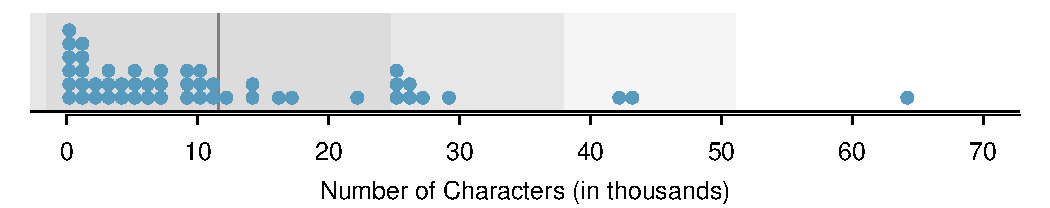
\includegraphics[width=\textwidth]{ch_summarizing_data/figures/emailCharactersDotPlot/emailCharactersDotPlotStackedRoundedWithSD}
\caption{In the \var{num\_\hspace{0.3mm}char} data, 40 of the 50 emails (80\%) are within 1~standard deviation of the mean, and 47 of the 50 emails (94\%) are within 2 standard deviations. Usually about 68\% (or approximately 2/3) of the data are within 1 standard deviation of the mean and 95\% are within 2 standard deviations, though this rule of thumb is less accurate for skewed data, as shown in this example.}
\label{emailCharactersDotPlotStackedRoundedWithSD}
\end{figure}

\Comment{We had gone through similar attempts early in OS on the changes being proposed in the tip box. On the 2nd and third sentences, which are new:
\begin{itemize}
\item The second sentence says almost nothing, and a simple distribution that students will consider in the course (binary where $p = 0.5$) also contradicts this guideline.
\item The third sentence is not true: the observations are not 1 SD away from the mean on average.
\end{itemize}}

\begin{tipBox}{\tipBoxTitle{standard deviation describes variability}{\color{red}ADD THIS BOX}
Focus on the conceptual meaning of the standard deviation as a descriptor of variability rather than the formulas. In general, some values will be more than one standard deviation from the mean and some values will be less than one standard deviation from the mean. However, \textit{on average}, the values will be one standard deviation from the mean.}
\end{tipBox}

\begin{tipBox}{\tipBoxTitle{standard deviation describes variability}{\color{red}CUT THIS BOX}
Focus on the conceptual meaning of the standard deviation as a descriptor of variability rather than the formulas. The empirical rule tells us that usually about 68\% of the data will be within one standard deviation of the mean and about 95\% will be within two standard deviations of the mean. However, as seen in Figures~\ref{emailCharactersDotPlotStackedRoundedWithSD} and~\ref{severalDiffDistWithSdOf1}, these percentages are not strict rules.\footnotemark}\footnotetext{We will learn where these two numbers come from in Chapter 4 when we study the normal distribution.}
\end{tipBox}

\Add{
The \term{empirical rule} tells us that usually about 68\% of the data will be within one standard deviation of the mean and about 95\% will be within two standard deviations of the mean. However, as seen in Figures~\ref{emailCharactersDotPlotStackedRoundedWithSD} and~\ref{severalDiffDistWithSdOf1}, these percentages are not strict rules.\footnote{We will learn where these two numbers come from in Chapter 4 when we study the normal distribution.}
}

\begin{figure}
\centering
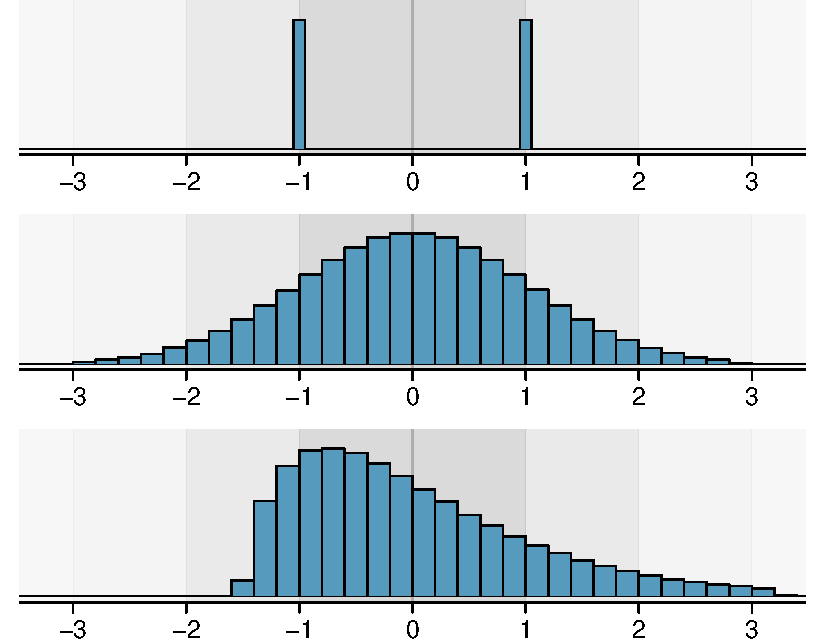
\includegraphics[width=0.65\textwidth]{ch_summarizing_data/figures/severalDiffDistWithSdOf1/severalDiffDistWithSdOf1}
\caption{Three very different population distributions with the same mean $\mu=0$ and standard deviation $\sigma=1$.}
\label{severalDiffDistWithSdOf1}
\end{figure}

\begin{exercise}
On page~\pageref{shapeFirstDiscussed}, the concept of shape of a distribution was introduced. A good description of the shape of a distribution should include modality and whether the distribution is symmetric or skewed to one side. Using Figure~\ref{severalDiffDistWithSdOf1} as an example, explain why such a description is important.\footnote{Figure~\ref{severalDiffDistWithSdOf1} shows three distributions that look quite different, but all have the same mean, variance, and standard deviation. Using modality, we can distinguish between the first plot (bimodal) and the last two (unimodal). Using skewness, we can distinguish between the last plot (right skewed) and the first two. While a picture, like a histogram, tells a more complete story, we can use modality and shape (symmetry/skew) to characterize basic information about a~distribution.}
\end{exercise}

\Add{
\begin{example}{Earlier we reported that the mean family income in the U.S. in 2012 was \$82,743. Estimating the standard deviation of income as approximately \$50,000, is a family income of \$60,000 unusually far from the mean or relatively close to the mean?}
Because \$60,000 is less that one standard deviation from the mean, it is relatively close to the mean. \Comment{I think this example can create confusion: it suggests that 1 SD is our rule for what is ``unusual'', when generally the rule of thumb is 2 SD.}
\end{example}
}

When describing any distribution, comment on the three important characteristics of center, spread, and shape. Also note any especially unusual cases.

\begin{example}{In the data's context (the number of characters in emails), describe the distribution of the \var{num\_\hspace{0.3mm}char} variable using the histogram in Figure~\ref{email50NumCharHistCopy}.}
The distribution of email character counts is unimodal and very strongly skewed to the right. Many of the counts fall near the mean at 11,600, and most fall within one standard deviation (13,130) of the mean. There is one exceptionally long email with about 65,000 characters.

\begin{figure}[ht]
   \centering
   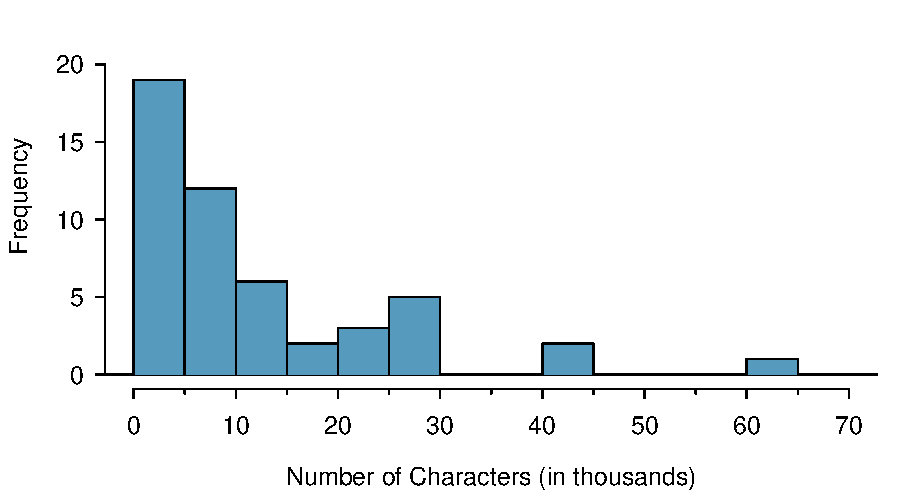
\includegraphics[width=0.8\textwidth]{ch_summarizing_data/figures/email50NumCharHist/email50NumCharHist}
   \caption{A copy of Figure~\ref{email50NumCharHist}.}
   \label{email50NumCharHistCopy}
\end{figure}

\end{example}

In this chapter we use standard deviation as a descriptive statistic to describe the variability in a given data set. In Chapter~\ref{foundationsForInference} we will use the standard deviation to assess how close a sample mean is to the population mean.

%\Comment{insert section on z-score? It doesn't quite fit into this section, but if we wait until we introduce the normal curve, then students think that z-scores always refer to normal distribution.}


\subsection{Box plots and quartiles}

A \term{box plot} summarizes a data set using five summary statistics while also plotting unusual observations. Figure~\ref{boxPlotLayoutNumVar} provides a box plot of the \var{num\_\hspace{0.3mm}char} variable from the \data{email50} data set.

\begin{figure}[h]
   \centering
   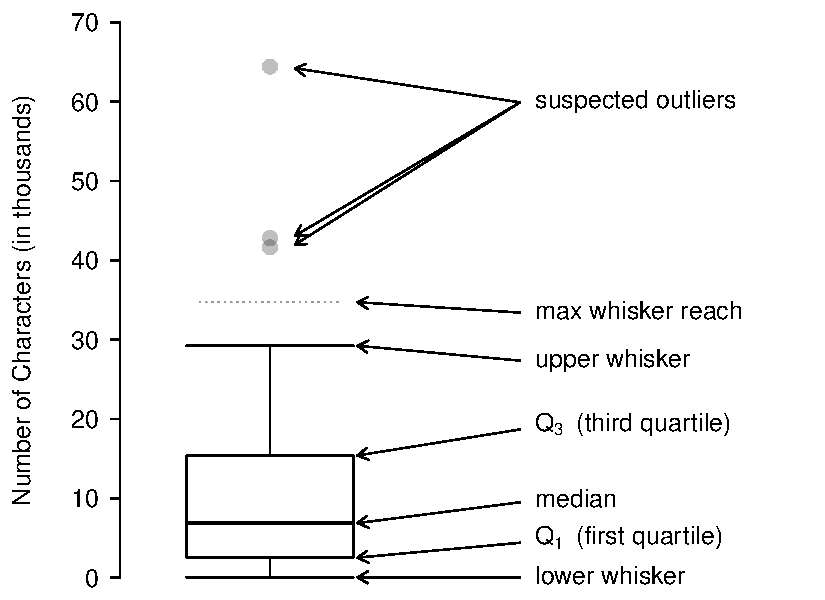
\includegraphics[width=0.85\mycaptionwidth]{ch_summarizing_data/figures/boxPlotLayoutNumVar/boxPlotLayoutNumVar}
\caption{A labeled box plot for the nuber of characters in 50 emails. The median (6,890) splits the data into the bottom 50\% and the top 50\%.}
  % \caption{A vertical dot plot next to a labeled box plot for the number of characters in 50 emails. The median (6,890), splits the data into the bottom 50\% and the top 50\%, marked in the dot plot by horizontal dashes and open circles, respectively.}
   \label{boxPlotLayoutNumVar}
\end{figure}

The five summary statistics used in a box plot are known as the \term{five-number summary}, which consists of the minimum, the maximum, and the three quartiles ($Q_1$, $Q_2$, $Q_3$) of the data set being studied.

$Q_2$\index{Q$_2$} represents the \term{second quartile}, which is equivalent to the 50th percentile (i.e. the median). Previously, we saw that Q$_2$ (the median) for the \data{email50} data set was the average of the two middle values: $\frac{\text{6,768} + \text{7,012}}{2} = \text{6,890}$.

$Q_1$\index{Q$_1$} represents the \term{first quartile}, which is the 25th percentile, and is the median of the smaller half of the data set. There are 25 values in the lower half of the data set, so $Q_1$ is the middle value: 2,454 characters. $Q_3$\index{$Q_3$} represents the \term{third quartile}, or 75th percentile, and is the median of the larger half of the data set: 15,829 characters.

To determine if there are any unusually distant observations (i.e. outliers), we first calculate the spread of the middle 50\% of the data by subtracting $Q_1$ from $Q_3$: $Q_3 - Q_1 = \text{13,375}$. This quantity is called the \term{interquartile range} (\hiddenterm{IQR}, for short). It, like the standard deviation, is a measure of \indexthis{variability}{variability} or \term{spread} in data. The more variable the data, the larger the standard deviation and~IQR tend to be.

\begin{termBox}{\tBoxTitle{Interquartile range (IQR)}
The IQR\index{interquartile range} is the length of the box in a box plot. It is computed as
\begin{eqnarray*}
IQR = Q_3 - Q_1
\end{eqnarray*}
where $Q_1$ and $Q_3$ are the $25^{th}$ and $75^{th}$ percentiles.}
\end{termBox}

To build a box plot, draw an axis (vertical or horizontal) and mark a uniform scale. Then, draw a dark line denoting $Q_2$. Next, draw a line at $Q_1$ and at $Q_3$. Connect these two lines to form a rectangle. The width of the rectangle corresponds to the IQR and the middle 50\% of the data is in this interval.

\Comment{The proposed updates here need work. For example, the first sentence says the whiskers suggest the whiskers reach out to the max and min values. What is broken about the original description?} \Add{Now the whiskers extend out on either end to the minimum and maximum values. However, if there are outliers, then we denote those outliers with a special symbol (a dot or an asterisk), and extend the whiskers to the smallest and largest values in the data set that are not outliers. Here, we define an outlier as a value that is more than $1.5\times IQR$ below $Q_1$ or above $Q_3$.\footnote{While the choice of exactly 1.5 is arbitrary, it is the most commonly used value for box plots.}  In Figure~\ref{boxPlotLayoutNumVar}, the upper whisker does not extend to the last three points, which are beyond $Q_3 + 1.5\times IQR$, and so it extends only to the last point below this limit. There are no values below $Q_1 - 1.5\times IQR$j, so the lower whisker stops at the minimum. In a sense, the box is like the body of the box plot and the whiskers are like its arms trying to reach the rest of the data, with outliers escaping their reach.} 
\Cut{
Extending out from the rectangle, the \term{whiskers} attempt to capture the data remaining outside of the box; however, their reach cannot be more than $1.5\times IQR$. In Figure~\ref{boxPlotLayoutNumVar}, the upper whisker does not extend to the last three points, which are beyond $Q_3 + 1.5\times IQR$, and so it extends only to the last point below this limit. The lower whisker stops at the lowest value, 33, since there is no additional data to reach. In a sense, the box is like the body of the box plot and the whiskers are like its arms trying to reach the rest of the data. We will call a value an \hiddenterm{outlier} if it is more than $1.5\times IQR$ below $Q_1$ or above $Q_3$.\footnote{While the choice of exactly 1.5 is arbitrary, it is the most commonly used value for box plots.}
}

\begin{example}{Compare the box plot to the graphs previously discussed: stem-and-leaf plot, dot plot, frequency and relative frequency histogram. What can we learn more easily from a box plot? What can we learn more easily from the other graphs?}
It is easier to immediately identify the quartiles from a box plot. The box plot also more prominently highlights outliers. However, a box plot, unlike the other graphs, does not show the \emph{distribution} of the data. For example, we cannot generally identify modes using a box plot.
\end{example}

\begin{example}
{Is it possible to identify skew from the box plot?} Yes. Looking at the lower and upper whiskers of this box plot, we see that the lower 25\% of the data is squished into a shorter distance than the upper 25\% of the data, implying that there is greater density in the low values and a tail trailing to the upper values. This box plot is right skewed.
\end{example}

\begin{exercise}
True or false: there is more data between the median and $Q_3$ than between $Q_1$ and the median.\footnote{False. Since $Q_1$ is the 25th percentile and the median is the 50th percentile, 25\% of the data fall between $Q_1$ and the median. Similarly, 25\% of the data fall between $Q_2$ and the median. The distance between the median and $Q_3$ is larger because that 25\% of the data is more spread out.}
\end{exercise}

%\Comment{TODO(David)  create another box plot using different data set}
%\Comment{TODO(Leah) redo exercise}

%\Cut{
%\begin{exercise}
%Using Figure~\ref{boxPlotLayoutNumVar}, estimate the following values for \var{num\_\hspace{0.3mm}char} in the \data{email50} data set: (a) $Q_1$, (b) $Q_3$, and (c) IQR.\footnote{These visual estimates will vary a little from one person to the next: $Q_1=$ 3,000, $Q_3=$ 15,000, $\text{IQR}=Q_3 - Q_1 = $ 12,000. (The true values: $Q_1=$ 2,536, $Q_3=$ 15,411, $\text{IQR} = $ 12,875.)}
%\end{exercise}
%}


\subsection{Calculator: summarize 1-variable statistics\textPE{\vspace{-3mm}}}
\label{TIsummarizedata}

\Comment{Change all \"TI calculator" headings to \"TI-84 calculator"?}

\begin{termBox}{\tBoxTitle{TI calculator:  Entering data}
The first step in summarizing data or making a graph is to  enter the data set into a list. Use \textbf{STAT, Edit}.
\begin{enumerate}
\item Press STAT.
\item Choose 1:Edit.
\item Enter data into L1 or another list.
\end{enumerate}
}
\end{termBox}

\begin{termBox}{\tBoxTitle{TI calculator:  Calculating Summary Statistics}
Use the \textbf{STAT, CALC, 1-VarStats} command to find summary statistics such as mean, standard deviation, and quartiles.
\begin{enumerate}
\setlength{\itemsep}{0mm}
\item Enter the data as described previously.
\item Press STAT.
\item Right arrow to CALC.
\item Choose 1:1-VarStats.
\item Enter L1 (i.e. 2ND 1) for List. If the data is in a list other than L1, type the name of that list.
\item Leave FreqList blank.
\item Choose Calculate and hit ENTER.
\begin{itemize}
\item[TI-83: ] Do steps 1-4, then type L1 (i.e. 2nd 1) or the name of your list and hit ENTER.
\end{itemize}
\end{enumerate}
}
\end{termBox}

Calculating the summary statistics will return the following information. It will be necessary to hit the down arrow to see all of the summary statistics.
\Comment{The max got cut off in last version, so added it in, which requires an extra line. May mess up formatting}

\begin{center}
\begin{tabular}{ll ll}
$\bar{\text{x}}$ & (mean)
	& minX & (minimum) \\
$\Sigma$x & (sum of all the data values)
	& Q$_1$ & (first quartile) \\
$\Sigma$x$^2$ & (sum of all the squared data values)
	& Med & (median)\\
$\sigma$x & (population standard deviation)
	& maxX & (maximum) \\
n & (sample size or \# of data points)
\end{tabular}
\end{center}

\begin{termBox}{\tBoxTitle{TI calculator:  Drawing a box plot}
Occasionally, we may want just a quick sketch of the box plot. In these instances we can use the graphing calculator to speed up the process. Use \textbf{2ND Y=}.
\begin{enumerate}
\item Enter the data to be graphed as described previously.
\item Hit 2ND Y= (i.e. STAT PLOT).
\item Hit Enter (to choose the first plot).
\item Hit ENTER to choose ON.
\item Down arrow and then right arrow three times to select box plot with outliers.
\item Down arrow again and make Xlist: L1 and Freq: 1.
\item Choose ZOOM and then 9:ZoomStat (to get a good viewing window).
\end{enumerate}
}
\end{termBox}

\begin{example}{Enter the following 10 data points into list L1 on a calculator: {5, 8, 1, 19, 3, 1, 11, 18, 20, 5}. Find the summary statistics and make a box plot of the data.}The summary statistics should be $\bar{\text{x}}$=9.1, Sx = 7.475, Q1 = 3, etc. The box plot should be as follows.	
\begin{center}
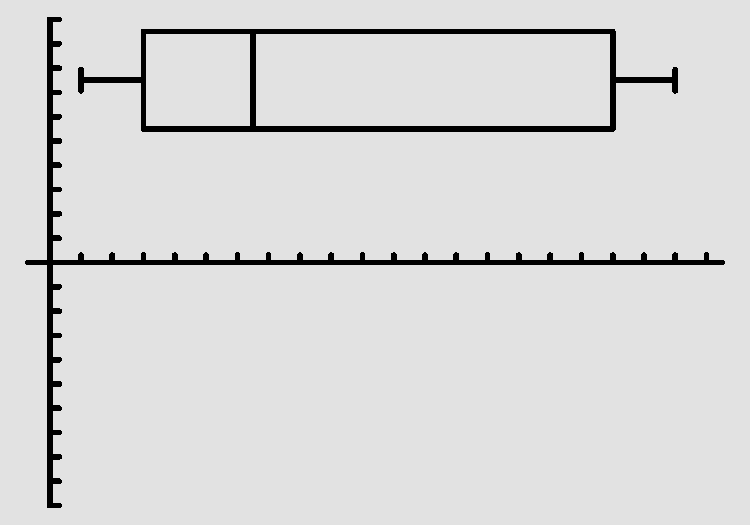
\includegraphics[width=0.45\textwidth]{ch_summarizing_data/figures/TI83_box_plot_A/TI83_box_plot_A}
\end{center}
\end{example}

%\CommentA{added tipbox}

\begin{tipBox}{\tipBoxTitle[]{TI calculator: What to do if you cannot find L1 or another list\vspace{-5mm}}
\begin{enumerate}
\setlength{\itemsep}{0mm}
\item Press STAT.
\item Choose 5: SetUpEditor.
\item Hit ENTER
\end{enumerate}
\quad Lists L1 - L6 will now be restored.}
\end{tipBox}


\subsection{Outliers and robust statistics\textPE{\vspace{-3mm}}}

\begin{termBox}{\tBoxTitle{Rules of thumb for identifying outliers}
There are two rules of thumb for identifying outliers:
\begin{itemize}
\setlength{\itemsep}{0mm}
\item More than 1.5$\times$ IQR below $Q_1$ or above $Q_3$
\item More than 2 standard deviations above or below the mean.
\end{itemize}
Both are important for the AP exam. In practice, consider these to be only rough guidelines.}
\end{termBox}

\begin{exercise}For the \data{email50} data set,$Q_1=$ 2,536 and $Q_3=15,411$. $\bar{x}$ = 11,600  and $s$ = 13,130. What values would be considered an outlier on the low end using each rule?\footnote{ $Q_1 - 1.5\times IQR = 2536 - 1.5 \times (15411 - 2536) = -16,749.5$, so values less than -16,749.5 would be considered an outlier using the first rule of thumb. Using the second rule of thumb, a value less than $\bar{x} - 2\times s = 11,600 - 2 \times 13,130 = -14,660$ would be considered an outlier. Note tht these are just rules of thumb and yield different values.}
\end{exercise}

\begin{exercise} Because there are no negative values in this data set, there can be no outliers on the low end. What does the fact that there are outliers on the high end but not on the low end suggestion?\footnote{It suggests that the distribution has a right hand tail, that~is, that it is right skewed.}
\end{exercise}

How are the \indexthis{sample statistics}{sample statistic} of the \data{num\_\hspace{0.3mm}char} data set affected by the observation, 64,401? What would have happened if this email wasn't observed? What would happen to these \indexthis{summary statistics}{summary statistic} if the observation at 64,401 had been even larger, say 150,000? These scenarios are plotted alongside the original data in Figure~\ref{email50NumCharDotPlotRobustEx}, and sample statistics are computed under each scenario in Table~\ref{robustOrNotTable}.

\begin{figure}[ht]
\centering
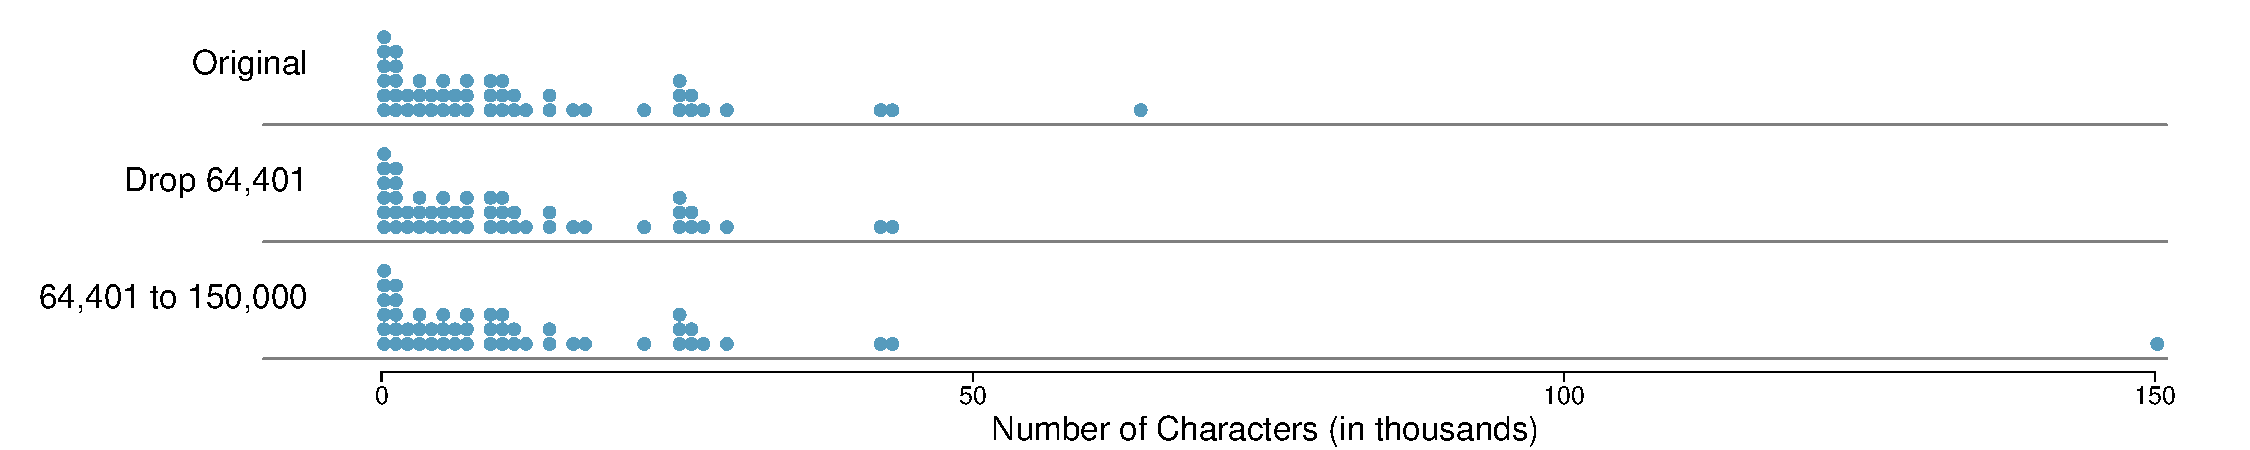
\includegraphics[width=\textwidth]{ch_summarizing_data/figures/emailCharactersDotPlot/email50NumCharDotPlotRobustEx}
\caption{Dot plots of the original character count data and two modified data sets.}
\label{email50NumCharDotPlotRobustEx}
\end{figure}

\begin{table}[ht]
\centering
\begin{tabular}{l c cc c cc}
  \hline
& \hspace{0mm} & \multicolumn{2}{c}{\bf robust} & \hspace{2mm} & \multicolumn{2}{c}{\bf not robust} \\
scenario && median & IQR && $\bar{x}$ & $s$ \\
  \hline
original \var{num\_\hspace{0.3mm}char} data 	&& 6,890 & 12,875 && 11,600 & 13,130 \\
% library(openintro); data(email50); d <- email50$num_char; median(d); diff(quantile(d, c(0.25,0.75))); mean(d); sd(d)
drop 66,924 observation		&& 6,768 & 11,702 && 10,521 & 10,798 \\
% library(openintro); data(email50); d <- email50$num_char; d <- d[-which.max(d)]; median(d); diff(quantile(d, c(0.25,0.75))); mean(d); sd(d)
move 66,924 to 150,000		&& 6,890 & 12,875 && 13,310 & 22,434 \\
% library(openintro); data(email50); d <- email50$num_char; d[which.max(d)] <- 100000; median(d); diff(quantile(d, c(0.25,0.75))); mean(d); sd(d)
   \hline
\end{tabular}
\caption{A comparison of how the median, IQR, mean ($\bar{x}$), and standard deviation ($s$) change when extreme observations are present.}
\label{robustOrNotTable}
\end{table}

\begin{exercise} \label{numCharWhichIsMoreRobust}
(a) Which is more affected by extreme observations, the mean or median? Table~\ref{robustOrNotTable} may be helpful. (b) Is the standard deviation or IQR more affected by extreme observations?\footnote{(a) Mean is affected more. (b) Standard deviation is affected more. Complete explanations are provided in the material following Guided Practice~\ref{numCharWhichIsMoreRobust}.}
\end{exercise}

The median and IQR are called \term{robust estimates} because extreme observations have little effect on their values. The mean and standard deviation are much more affected by changes in extreme observations.

\begin{example}{The median and IQR do not change much under the three scenarios in Table~\ref{robustOrNotTable}. Why might this be the case?}
Since there are no large gaps between observations around the three quartiles, adding, deleting, or changing one value, no matter how extreme that value, will have little effect on their values.
\end{example}

\begin{exercise}
The distribution of vehicle prices tends to be right skewed, with a few luxury and sports cars lingering out into the right tail. If you were searching for a new car and cared about price, should you be more interested in the mean or median price of vehicles sold, assuming you are in the market for a regular car?\footnote{Buyers of a ``regular car'' should be concerned about the median price. High-end car sales can drastically inflate the mean price while the median will be more robust to the influence of those sales.}
\end{exercise}


\subsection{Linear transformations of data}
\label{linearTransformationOfData}

\begin{example}{Begin with the following list:  {1, 1, 5, 5}. Multiply all of the numbers by 10. What happens to the mean? What happens to the standard deviation? How do these compare to the mean and the standard deviation of the original list?}
The original list has a mean of 3 and a standard deviation of 2. The new list: {10, 10, 50, 50} has a mean of 30 with a standard deviation of 20. Because all of the values were multiplied by 10, both the mean and the standard deviation were multiplied by~10.~\footnote{Here, the population standard deviation was used in the calculation. These properties can be proven mathematically using properties of sigma (summation).}
\end{example}

\begin{example}{Start with the following list:  {1, 1, 5, 5}. Multiply all of the numbers by \mbox{-0.5}. What happens to the mean? What happens to the standard deviation? How do these compare to the mean and the standard deviation of the original list?}
The new list: {-0.5, -0.5, -2.5, -2.5} has a mean of -1.5 with a standard deviation of~1. Because all of the values were multiplied by~\mbox{-0.5}, the mean was multiplied by~\mbox{-0.5}. Multiplying all of the values by a negative flipped the sign of numbers, which affects the location of the center, but not the spread. Multiplying all of the values by \mbox{-0.5} multiplied the standard deviation by +0.5 since the standard deviation cannot be negative.
\end{example}

\begin{example}{Again, start with the following list: {1, 1, 5, 5}. Add 100 to every entry. How do the new mean and standard deviation compare to the original mean and standard deviation?}
The new list is: {101, 101, 105, 105}. The new mean of 103 is 100 greater than the original mean of 3. The new standard deviation of 2 is the \emph{same} as the original standard deviation of 2. Adding a constant to every entry shifted the values, but did not stretch them.
\end{example}

Suppose that a researcher is looking at a list of 500 temperatures recorded in Celsius~(C). The mean of the temperatures listed is given as 27\degree C with a standard deviation of 3\degree C. Because she is not familiar with the Celsius scale, she would like to convert these summary statistics into Fahrenheit~(F). To convert from Celsius to Fahrenheit, we use the following conversion:
\begin{align*}
x_{_F} = \frac{9}{5}x_{_C} + 32
\end{align*}
Fortunately, she does not need to convert each of the 500 temperatures to Fahrenheit and then recalculate the mean and the standard deviation. The unit conversion above is a linear transformation of the following form, where $a=9/5$ and $b=32$:
\begin{align*}
aX + b
\end{align*}
Using the examples as a guide, we can solve this temperature-conversion problem. The mean was 27\degree C and the standard deviation was 3\degree C. To convert to Fahrenheit, we multiply all of the values by $9/5$, which multiplies both the mean and the standard deviation by $9/5$. Then we add 32 to all of the values which adds 32 to the mean but does not change the standard deviation further.
\begin{align*}
\bar{x}_{F} &= \frac{9}{5}\bar{x}_{C} + 32 & \sigma_{F} &= \frac{9}{5}\sigma_{C} \\
&= \frac{5}{9}(27)+ 32 & &=\frac{9}{5}(3) \\
&=80.6 &  &=5.4
\end{align*}

\begin{figure}[h]
   \centering
   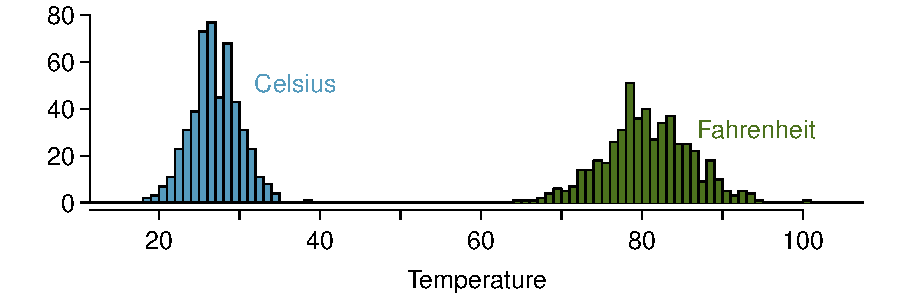
\includegraphics[width=0.9\textwidth]{ch_summarizing_data/figures/CToF_ConversionFigure/CToF_ConversionFigure}
   \caption{500 temperatures shown in both Celsius and \mbox{Fahrenheit.}}
   \label{CToF_ConversionFigure}
\end{figure}

%\Comment{TODO(David) THIS WOULD BE NICE add picture}

\begin{termBox}{\tBoxTitle{Adding shifts the values, multiplying stretches or contracts them}
Adding a constant to every value in a data set shifts the mean but does not affect the standard deviation. Multiplying the values in a data set by a constant will change the mean and the standard deviation by the same multiple, except that the standard deviation will always remain positive.}
\end{termBox}

\begin{example}{Consider the temperature example. How would converting from Celsuis to Fahrenheit affect the median? The IQR?}
The median is affected in the same way as the mean and the IQR is affected in the same way as the standard deviation. To get the new median, multiply the old median by $9/5$ and add 32. The IQR is computed by subtracting $Q_1$ from $Q_3$. While $Q_1$ and $Q_3$ are each affected in the same way as the median, the additional 32 added to each will cancel when we take $Q_3 - Q_1$. That is, the IQR will be increase by a factor of $9/5$ but will be unaffected by the addition of~32.

For a more mathematical explanation of the IQR calculation, see the footnote.\footnote{new IQR = $\left(\frac{9}{5} Q_3 + 32\right) - \left(\frac{9}{5} Q_1 + 32\right) = \frac{9}{5} \left(Q_3 - Q_1\right) = \frac{9}{5} \times \text{(old IQR)}$.}
\end{example}

\subsection{Comparing numerical data across groups}
\label{comparingAcrossGroups}

\index{data!county|(}

%\Comment{TODO(David) add back-to-back stem-and-leaf. THIS CHANGE IS NECESSARY.}

Some of the more interesting investigations can be considered by examining numerical data across groups. The methods required here aren't really new. All that is required is to make a numerical plot for each group. To make a direct comparison between two groups, create a pair of dot plots or a pair of histograms drawn using the same scales. It is also common to use back-to-back stem-and-leaf plots, parallel box plots, and hollow histograms, the three of which are explored here.

We will take a look again at the \data{county} data set and compare the median household income for counties that gained population from 2000 to 2010 versus counties that had no gain. While we might like to make a causal connection here, remember that these are observational data and so such an interpretation would be unjustified.

There were 2,041 counties where the population increased from 2000 to 2010, and there were 1,099 counties with no gain (all but one were a loss). A~random sample of 100 counties from the first group and 50 from the second group are shown in Table~\ref{countyIncomeSplitByPopGainTable} to give a better sense of some of the raw data, and Figure~\ref{stemandleafincomepopgainloss} shows a \termsub{back-to-back stem-and-leaf plot}{stem-and-leaf plot!back-to-back}.

\begin{table}
\centering
\begin{tabular}{ ccc ccc c ccc }
\multicolumn{6}{c}{\bf population gain} && \multicolumn{3}{c}{\bf no gain} \\
  \cline{1-6} \cline{8-10}
41.2 & 33.1 & 30.4 & 37.3 & 79.1 & 34.5 &\hspace{5mm}\ & 40.3 & 33.5 & 34.8 \\
22.9 & 39.9 & 31.4 & 45.1 & 50.6 & 59.4 && 29.5 & 31.8 & 41.3 \\
47.9 & 36.4 & 42.2 & 43.2 & 31.8 & 36.9 && 28 & 39.1 & 42.8 \\
50.1 & 27.3 & 37.5 & 53.5 & 26.1 & 57.2 && 38.1 & 39.5 & 22.3 \\
57.4 & 42.6 & 40.6 & 48.8 & 28.1 & 29.4 && 43.3 & 37.5 & 47.1 \\
43.8 & 26 & 33.8 & 35.7 & 38.5 & 42.3 && 43.7 & 36.7 & 36 \\
41.3 & 40.5 & 68.3 & 31 & 46.7 & 30.5 && 35.8 & 38.7 & 39.8 \\
68.3 & 48.3 & 38.7 & 62 & 37.6 & 32.2 && 46 & 42.3 & 48.2 \\
42.6 & 53.6 & 50.7 & 35.1 & 30.6 & 56.8 && 38.6 & 31.9 & 31.1 \\
66.4 & 41.4 & 34.3 & 38.9 & 37.3 & 41.7 && 37.6 & 29.3 & 30.1 \\
51.9 & 83.3 & 46.3 & 48.4 & 40.8 & 42.6 && 57.5 & 32.6 & 31.1 \\
44.5 & 34 & 48.7 & 45.2 & 34.7 & 32.2 && 46.2 & 26.5 & 40.1 \\
39.4 & 38.6 & 40 & 57.3 & 45.2 & 33.1 && 38.4 & 46.7 & 25.9 \\
43.8 & 71.7 & 45.1 & 32.2 & 63.3 & 54.7 && 36.4 & 41.5 & 45.7 \\
71.3 & 36.3 & 36.4 & 41 & 37 & 66.7 && 39.7 & 37 & 37.7 \\
50.2 & 45.8 & 45.7 & 60.2 & 53.1 &  && 21.4 & 29.3 & 50.1 \\
35.8 & 40.4 & 51.5 & 66.4 & 36.1 &  && 43.6 & 39.8 &  \\
\cline{1-6} \cline{8-10}
\end{tabular}
\caption{In this table, median household income (in \$1000s) from a random sample of 100 counties that gained population over 2000-2010 are shown on the left. Median incomes from a random sample of 50 counties that had no population gain are shown on the right.}
\label{countyIncomeSplitByPopGainTable}
\end{table}

\begin{figure}
\begin{verbatim}
           Population: Gain               Population: No Gain

                               3| 2 |12
                           98766| 2 |66899
                 444433222211100| 3 |00112234
             9999888777766666655| 3 |56667788888999
            44433332221111110000| 4 |0000001223344
                   9988876665555| 4 |666778
                       443221100| 5 |0
                          977775| 5 |8
                             320| 6 |
                           88766| 6 |
                              21| 7 |

            Legend: 4 | 5 = 45,000 median income
\end{verbatim}
\caption{Back-to-back stem-and-leaf plot for median income, split by whether the count had a population gain or no gain.}
\label{stemandleafincomepopgainloss}
\end{figure}

The \term{parallel box plot} \index{box plot!parallel box plot} is a traditional tool for comparing across groups. An example is shown in the left panel of Figure~\ref{countyIncomeSplitByPopGain}, where there are two box plots, one for each group, placed into one plotting window and drawn on the same scale.

\begin{figure}
   \centering
   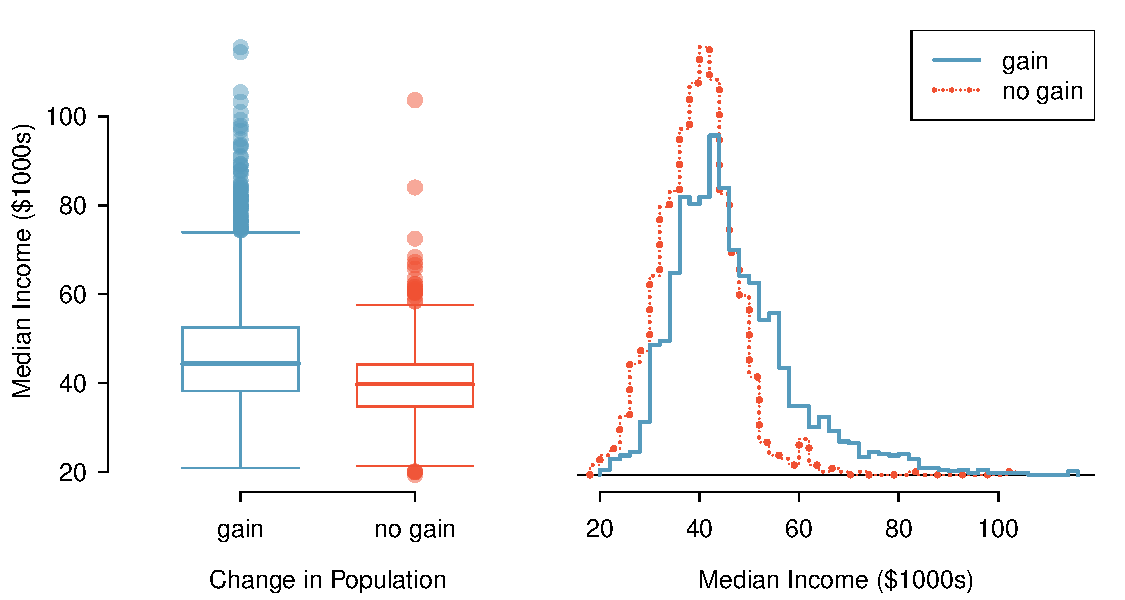
\includegraphics[width=\textwidth]{ch_summarizing_data/figures/countyIncomeSplitByPopGain/countyIncomeSplitByPopGain}
   \caption{Side-by-side box plot (left panel) and hollow histograms (right panel) for \var{med\_\hspace{0.3mm}income}, where the counties are split by whether there was a population gain or loss from 2000 to 2010. The income data were collected between 2006 and 2010.}
   \label{countyIncomeSplitByPopGain}
\end{figure}

Another useful plotting method uses \termsub{hollow histograms}{hollow histogram} to compare numerical data across groups. These are just the outlines of histograms of each group put on the same plot, as shown in the right panel of Figure~\ref{countyIncomeSplitByPopGain}.

\begin{exercise} \label{comparingPriceByTypeExercise}
Use the plots in Figure~\ref{countyIncomeSplitByPopGain} to compare the incomes for counties across the two groups. What do you notice about the approximate center of each group? What do you notice about the variability between groups? Is the shape relatively consistent between groups? How many \emph{prominent} modes are there for each group?\footnote{Answers may vary a little. The counties with population gains tend to have higher income (median of about \$45,000) versus counties without a gain (median of about \$40,000). The variability is also slightly larger for the population gain group. This is evident in the IQR, which is about 50\% bigger in the \emph{gain} group. Both distributions show slight to moderate right skew\index{skew!example: slight to moderate} and are unimodal. There is a secondary small bump at about \$60,000 for the \emph{no gain} group, visible in the hollow histogram plot, that seems out of place. (Looking into the data set, we would find that 8 of these 15 counties are in Alaska and Texas.) The box plots indicate there are many observations far above the median in each group, though we should anticipate that many observations will fall beyond the whiskers when using such a large data set.}
\end{exercise}

\begin{tipBox}{\tipBoxTitle{Comparing distributions}
When comparing distributions, compare them with respect to center, spread, and shape as well as any unusual observations. Such descriptions should be in context.}
\end{tipBox}

\begin{exercise}
What components of each plot in Figure~\ref{countyIncomeSplitByPopGain} do you find most useful?\footnote{Answers will vary. The parallel box plots are especially useful for comparing centers and spreads, while the hollow histograms are more useful for seeing distribution shape, skew, and groups of anomalies.}
\end{exercise}

\begin{exercise}
Do these graphs tell us about any association between income for the two groups?\footnote{No, to see association we require a scatterplot. Moreover, these data are not paired, so the discussion of association does not make sense here.}
\end{exercise}

\Comment{Adding a tip box below on the proposed topic sounds good, but it needs to be shorter. Try moving some of the content out of the box, or cut out some content.}

\begin{tipBox}{\tipBoxTitle{Comparing distributions versus looking at association}{\color{red}ADD THIS BOX}
To compare two distributions, we require two data sets that we can compare with respect to center and spread. The number of elements in each data set need not be the same (e.g. if comparing the height of men and women, we could have samples of different sizes). We must compare two univariate graphs, such as two histograms, two dot plots, parallel box plots, or a back-to-back stem-and-leaf. To look at association, we require two data sets of equal length that are essentially paired (e.g. height and weight of individuals). Such association can be seen in a scatterplot.}
\end{tipBox}


\index{data!email50|)}


\subsection{Mapping data (special topic)}

\index{intensity map|(}

The \data{county} data set offers many numerical variables that we could plot using dot plots, scatterplots, or box plots, but these miss the true nature of the data. Rather, when we encounter geographic data, we should map it using an \term{intensity map}, where colors are used to show higher and lower values of a variable. Figures~\ref{countyIntensityMaps1} and~\ref{countyIntensityMaps2} shows intensity maps for federal spending per capita (\var{fed\_\hspace{0.3mm}spend}), poverty rate in percent (\var{poverty}), homeownership rate in percent (\var{homeownership}), and median household income (\var{med\_\hspace{0.3mm}income}). The color key indicates which colors correspond to which values. Note that the intensity maps are not generally very helpful for getting precise values in any given county, but they are very helpful for seeing geographic trends and generating interesting research questions.

\begin{figure}
\centering
\subfigure[]{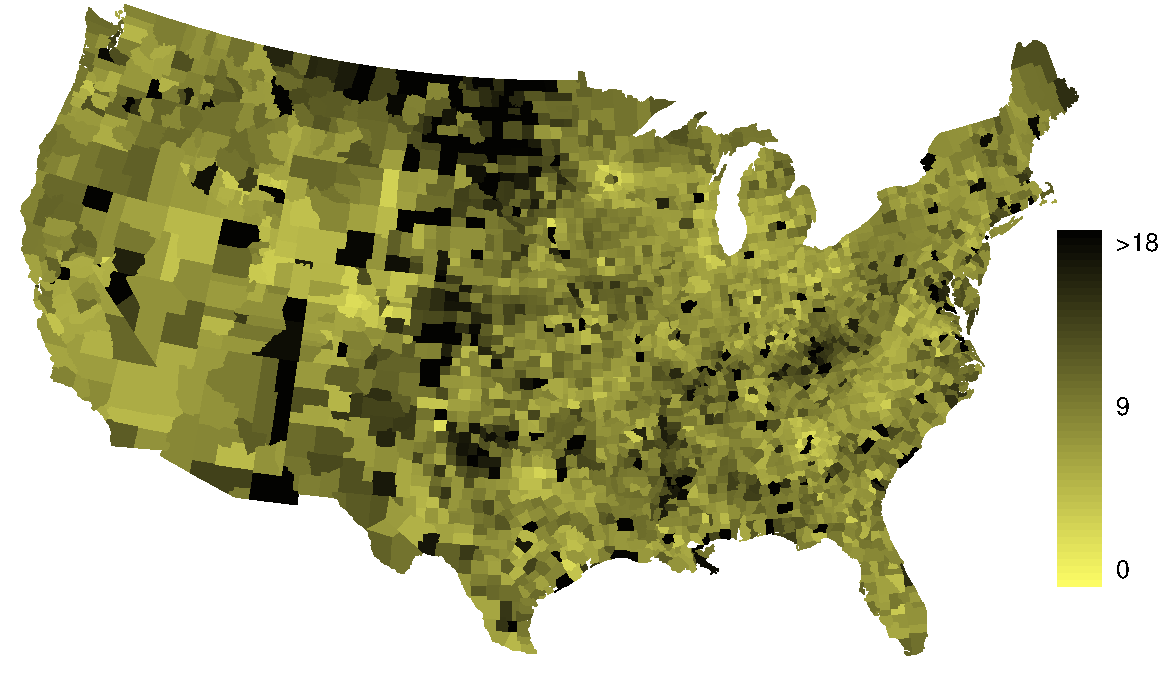
\includegraphics[width=\textwidth]{ch_summarizing_data/figures/countyIntensityMaps/countyFedSpendMap}\label{countyFedSpendMap}}
\subfigure[]{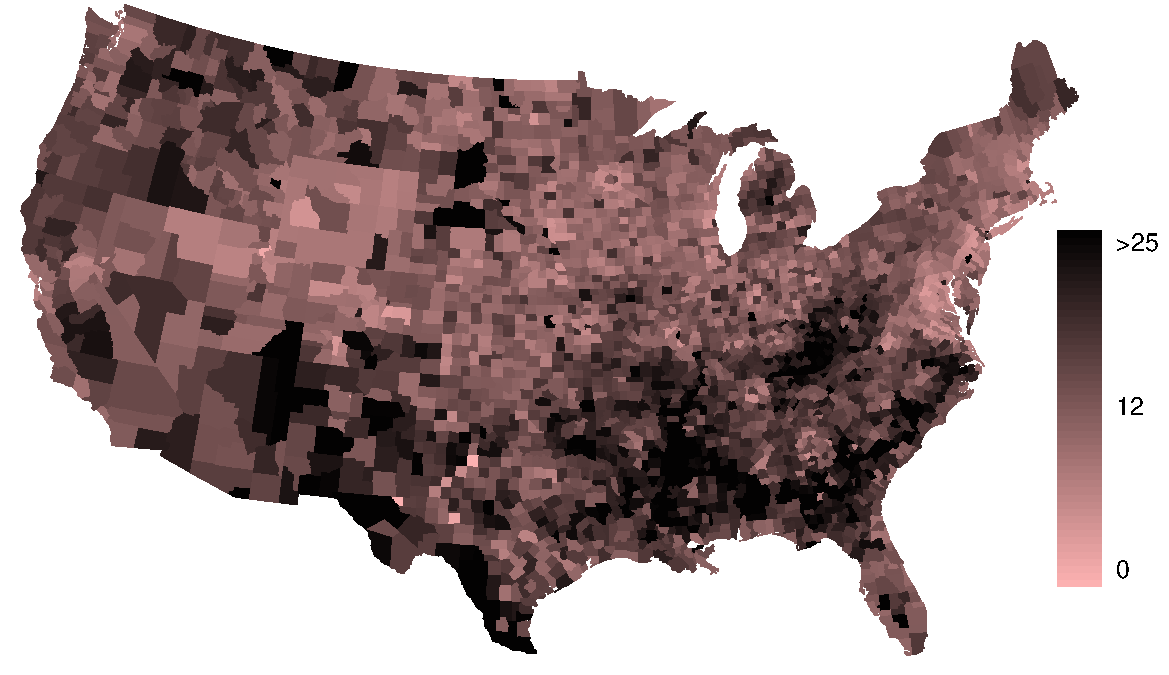
\includegraphics[width=\textwidth]{ch_summarizing_data/figures/countyIntensityMaps/countyPovertyMap}\label{countyPovertyMap}}
\caption{\subref{countyFedSpendMap} Map of federal spending (dollars per capita). \subref{countyPovertyMap} Intensity map of poverty rate (percent).}
\label{countyIntensityMaps1}
\end{figure}

\begin{figure}
\centering
\subfigure[]{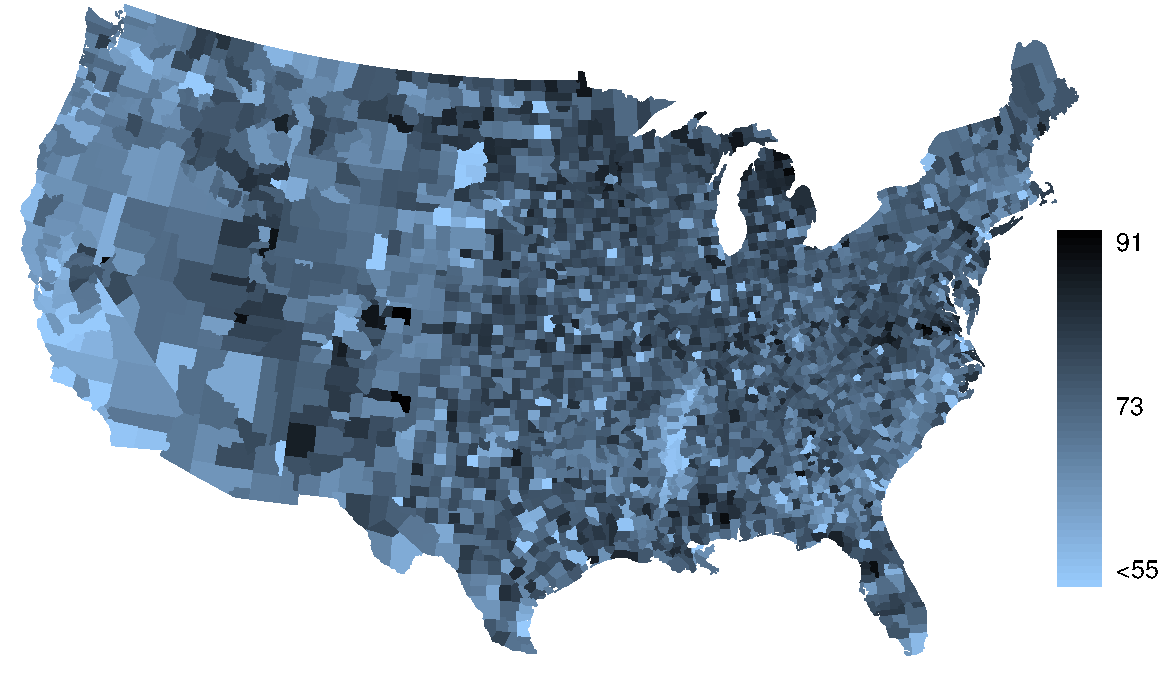
\includegraphics[width=\textwidth]{ch_summarizing_data/figures/countyIntensityMaps/countyHomeownershipMap}\label{countyHomeownershipMap}}
\subfigure[]{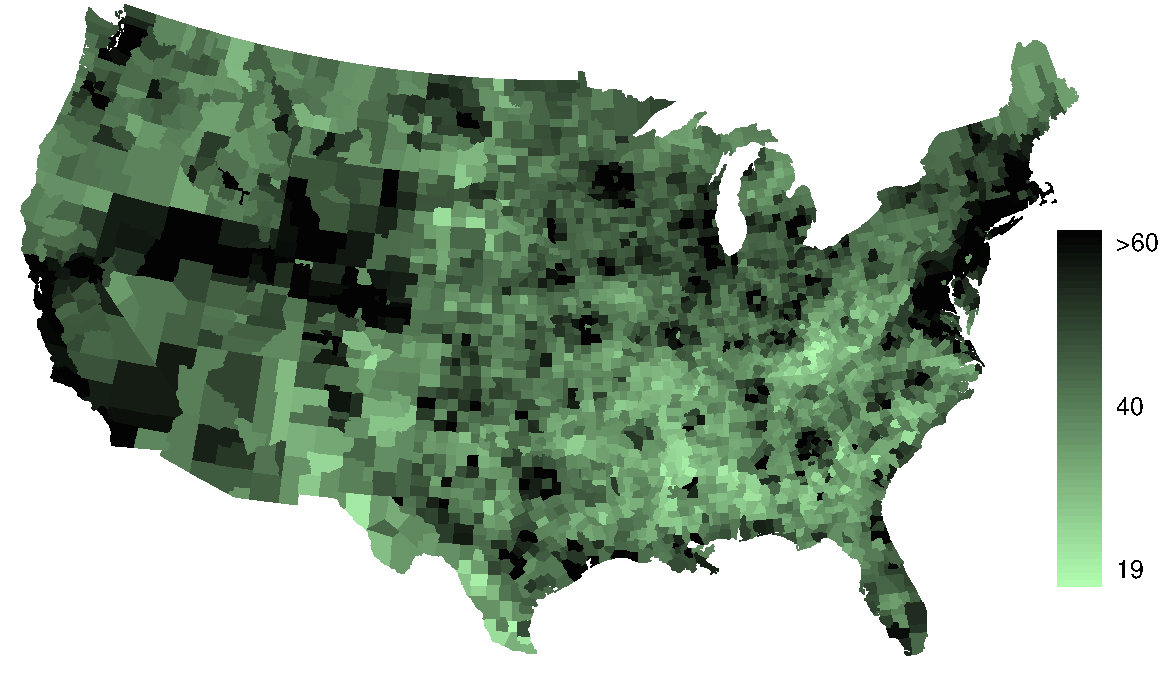
\includegraphics[width=\textwidth]{ch_summarizing_data/figures/countyIntensityMaps/countyMedIncomeMap}\label{countyMedIncomeMap}}
\caption{\subref{countyHomeownershipMap} Intensity map of homeownership rate (percent). \subref{countyMedIncomeMap} Intensity map of median household income (\$1000s).}
\label{countyIntensityMaps2}
\end{figure}

\begin{example}{What interesting features are evident in the \var{fed\_\hspace{0.3mm}spend} and \var{poverty} intensity maps?}
The federal spending intensity map shows substantial spending in the Dakotas and along the central-to-western part of the Canadian border, which may be related to the oil boom in this region. There are several other patches of federal spending, such as a vertical strip in eastern Utah and Arizona and the area where Colorado, Nebraska, and Kansas meet. There are also seemingly random counties with very high federal spending relative to their neighbors. If we did not cap the federal spending range at \$18 per capita, we would actually find that some counties have extremely high federal spending while there is almost no federal spending in the neighboring counties. These high-spending counties might contain military bases, companies with large government contracts, or other government facilities with many employees.

Poverty rates are evidently higher in a few locations. Notably, the deep south shows higher poverty rates, as does the southwest border of Texas. The vertical strip of eastern Utah and Arizona, noted above for its higher federal spending, also appears to have higher rates of poverty (though generally little correspondence is seen between the two variables). High poverty rates are evident in the Mississippi flood plains a little north of New Orleans and also in a large section of Kentucky and West Virginia.
\end{example}

\begin{exercise}
What interesting features are evident in the \var{med\_\hspace{0.3mm}income} intensity map?\footnote{Note: answers will vary. There is a very strong correspondence between high earning and metropolitan areas. You might look for large cities you are familiar with and try to spot them on the map as dark spots.}
\end{exercise}

\index{intensity map|)}
\index{data!county|)}


\section{Considering categorical data}
\label{categoricalData}

\index{data!email|(}

Like numerical data, categorical data can also be organized and analyzed. In this section, we will introduce tables and other basic tools for categorical data that are used throughout this book. The \data{email50} data set represents a sample from a larger email data set called \data{email}. This larger data set contains information on 3,921 emails. In this section we will examine whether the presence of numbers, small or large, in an email provides any useful value in classifying email as spam or not spam.
% library(openintro); data(email); dim(email)

\subsection{Contingency tables and bar plots}

Table~\ref{emailSpamNumberTableTotals} summarizes two variables: \var{spam} and \var{number}. Recall that \var{number} is a categorical variable that describes whether an email contains no numbers, only small numbers (values under 1 million), or at least one big number (a value of 1 million or more). A table that summarizes data for two categorical variables in this way is called a \term{contingency table}. Each value in the table represents the number of times a particular combination of variable outcomes occurred. For example, the value 149 corresponds to the number of emails in the data set that are spam \emph{and} had no number listed in the email. Row and column totals are also included. The \term{row totals} \index{contingency table!row totals} provide the total counts across each row (e.g. $149 + 168 + 50 = 367$), and \term{column totals} \index{contingency table!column totals} are total counts down each column.

Table~\ref{emailNumberTable} shows a frequency table for the \var{number} variable. If we replaced the counts with percentages or proportions, the table is a \term{relative frequency table}.

\begin{table}[ht]
\centering
\begin{tabular}{ll  ccc  rr}
& & \multicolumn{3}{c}{\bf \var{number}} & \\
  \cline{3-5}
& & none & small & big & Total & \hspace{2mm}\  \\
  \cline{2-6}
	 & spam &  149 & 168 &  50 & 367 \\
\raisebox{1.5ex}[0pt]{\var{spam}}
	& not spam &  400 & 2659 & 495 & 3554 \\
  \cline{2-6}
& Total & 549 & 2827 & 545 & 3921 \\
  \cline{2-6}
\end{tabular}
\caption{A contingency table for \var{spam} and \var{number}.}
\label{emailSpamNumberTableTotals}
%library(openintro); library(xtable); data(email); tab <- table(email[,c("spam", "number")])[2:1,]; xtable(tab); rowSums(tab); colSums(tab); sum(tab)
\end{table}

\begin{table}[htb]
\centering
\begin{tabular}{cccc}
  \hline
none & small & big & Total \\
 % \hline
 549 & 2827 & 545 & 3921 \\
   \hline
\end{tabular}
\caption{A frequency table for the \var{number} variable.}
\label{emailNumberTable}
\end{table}
%library(openintro); library(xtable); data(email); xtable(table(email[,c("html")]))

Because the numbers in these tables are counts, not to data points, they cannot be graphed using the methods we applied to numerical data. Instead, another set of graphing methods are needed that are suitable for categorical data.

A bar plot is a common way to display a single categorical variable. The left panel of Figure~\ref{emailNumberBarPlot} shows a \term{bar plot} for the \var{number} variable. In the right panel, the counts are converted into proportions (e.g. $549/3921=0.140$ for \resp{none}), showing the proportion of observations that are in each level (i.e. in each category).

\begin{figure}[bht]
   \centering
   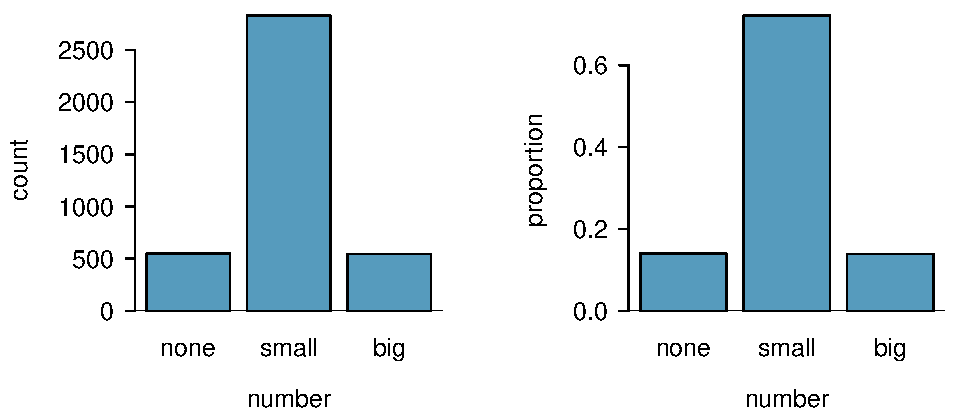
\includegraphics[height=2.3in]{ch_summarizing_data/figures/emailNumberBarPlot/emailNumberBarPlot}
   \caption{Two bar plots of \var{number}. The left panel shows the counts, and the right panel shows the proportions in each group.}
   \label{emailNumberBarPlot}
\end{figure}


\subsection{Row and column proportions}

Table~\ref{rowPropSpamNumber} shows the row proportions for Table~\ref{emailSpamNumberTableTotals}. The \termsub{row proportions}{contingency table!row proportions} are computed as the counts divided by their row totals. The value 149 at the intersection of \resp{spam} and \resp{none} is replaced by $149/367=0.406$, i.e. 149 divided by its row total, 367. So what does 0.406 represent? It corresponds to the proportion of spam emails in the sample that do not have any numbers.

\begin{table}[ht]
\centering
\begin{tabular}{l rrr r}
  \hline
 & none & small & big & Total \\
  \hline
spam &  $149/367 = 0.406$ & $168/367 = 0.458$ &
			$50/367 = 0.136$ & 1.000 \\
not spam &  $400/3554 = 0.113$ & $2657/3554 = 0.748$ &
			$495/3554 = 0.139$ & 1.000 \\
   \hline
Total & $549/3921 = 0.140$ & $2827/3921 = 0.721$ &
			$545/3921 = 0.139$ & 1.000 \\
  \hline
\end{tabular}
\caption{A contingency table with row proportions for the \var{spam} and \var{number} variables.}
\label{rowPropSpamNumber}
% library(openintro); data(email); g <- table(email$spam, email$number)[2:1,]; g / rep(rowSums(g), 3); rowSums(g)
\end{table}

A contingency table of the column proportions is computed in a similar way, where each \termsub{column proportion}{contingency table!column proportion} is computed as the count divided by the corresponding column total. Table~\ref{colPropSpamNumber} shows such a table, and here the value 0.271 indicates that 27.1\% of emails with no numbers were spam. This rate of spam is much higher compared to emails with only small numbers (5.9\%) or big numbers (9.2\%). Because these spam rates vary between the three levels of \var{number} (\resp{none}, \resp{small}, \resp{big}), this provides evidence that the \var{spam} and \var{number} variables are associated.

\begin{table}[ht]
\centering\small
\begin{tabular}{l rrr r}
  \hline
 & none & small & big & Total \\
  \hline
spam &  $149/549 = 0.271$ & $168/2827 = 0.059$ &
				$50/545 = 0.092$ & $367/3921 = 0.094$ \\
not spam &  $400/549 = 0.729$ & $2659/2827 = 0.941$ &
				$495/545 = 0.908$ & $3684/3921 = 0.906$ \\
   \hline
Total & 1.000 & 1.000 & 1.000 & 1.000 \\
   \hline
\end{tabular}
\caption{A contingency table with column proportions for the \var{spam} and \var{number} variables.}
\label{colPropSpamNumber}
% library(openintro); data(email); g <- table(email$spam, email$number)[2:1,]; g / rep(colSums(g), rep(2, 3)); g; colSums(g)
\end{table}

We could also have checked for an association between \var{spam} and \var{number} in Table~\ref{rowPropSpamNumber} using row proportions. When comparing these row proportions, we would look down columns to see if the fraction of emails with no numbers, small numbers, and big numbers varied from \resp{spam} to \resp{not~spam}.

\begin{exercise}
What does 0.458 represent in Table~\ref{rowPropSpamNumber}? What does 0.059 represent in Table~\ref{colPropSpamNumber}?\footnote{0.458 represents the proportion of spam emails that had a small number. 0.058 represents the fraction of emails with small numbers that are spam.}
\end{exercise}

\begin{exercise}
What does 0.139 at the intersection of \resp{not~spam} and \resp{big} represent in Table~\ref{rowPropSpamNumber}? What does 0.908 represent in the Table~\ref{colPropSpamNumber}?\footnote{0.139 represents the fraction of non-spam email that had a big number. 0.908 represents the fraction of emails with big numbers that are non-spam emails.}
\end{exercise}

\begin{example}{Data scientists use statistics to filter spam from incoming email messages. By noting specific characteristics of an email, a data scientist may be able to classify some emails as spam or not spam with high accuracy. One of those characteristics is whether the email contains no numbers, small numbers, or big numbers. Another characteristic is whether or not an email has any HTML content. A contingency table for the \var{spam} and \var{format} variables from the \data{email} data set are shown in Table~\ref{emailSpamHTMLTableTotals}. Recall that an HTML email is an email with the capacity for special formatting, e.g. bold text. In Table~\ref{emailSpamHTMLTableTotals}, which would be more helpful to someone hoping to classify email as spam or regular email: row or column proportions?}\label{weighingRowColumnProportions}
Such a person would be interested in how the proportion of spam changes within each email format. This corresponds to column proportions: the proportion of spam in plain text emails and the proportion of spam in HTML emails.

If we generate the column proportions, we can see that a higher fraction of plain text emails are spam ($209/1195 = 17.5\%$) than compared to HTML emails ($158/2726 = 5.8\%$). This information on its own is insufficient to classify an email as spam or not spam, as over 80\% of plain text emails are not spam. Yet, when we carefully combine this information with many other characteristics, such as \var{number} and other variables, we stand a reasonable chance of being able to classify some email as spam or not spam.
\end{example}

\begin{table}[ht]
\centering
\begin{tabular}{l cc r}
  \hline
 & text & HTML & Total \\
  \hline
spam & 209 & 158 & 367 \\
not spam & 986 & 2568 & 3554 \\
   \hline
Total & 1195 & 2726 & 3921 \\
   \hline
\end{tabular}
\caption{A contingency table for \var{spam} and \var{format}.}
\label{emailSpamHTMLTableTotals}
%library(openintro); library(xtable); data(email); tab <- table(email[,c("spam", "format")])[2:1,]; tab; colSums(tab); rowSums(tab)
\end{table}

Example~\ref{weighingRowColumnProportions} points out that row and column proportions are not equivalent. Before settling on one form for a table, it is important to consider each to ensure that the most useful table is constructed.

\begin{exercise}
Look back to Tables~\ref{rowPropSpamNumber} and~\ref{colPropSpamNumber}. Which would be more useful to someone hoping to identify spam emails using the \var{number} variable?\footnote{The column proportions in Table~\ref{colPropSpamNumber} will probably be most useful, which makes it easier to see that emails with small numbers are spam about 5.9\% of the time (relatively rare). We would also see that about 27.1\% of emails with no numbers are spam, and 9.2\% of emails with big numbers are spam.}
\end{exercise}


\subsection{Segmented bar plots}
\label{segmentedBarPlotsAndIndependence}

Contingency tables using row or column proportions are especially useful for examining how two categorical variables are related. Segmented bar plots provide a way to visualize the information in these tables.

A \termsub{segmented bar plot}{bar plot!segmented bar plot} is a graphical display of contingency table information. For example, a segmented bar plot representing Table~\ref{colPropSpamNumber} is shown in Figure~\ref{emailSpamNumberSegBar}, where we have first created a bar plot using the \var{number} variable and then divided each group by the levels of \var{spam}. The column proportions of Table~\ref{colPropSpamNumber} have been translated into a standardized segmented bar plot in Figure~\ref{emailSpamNumberSegBarSta}, which is a helpful visualization of the fraction of spam emails in each level of \var{number}.

\begin{figure}
\centering
\subfigure[]{
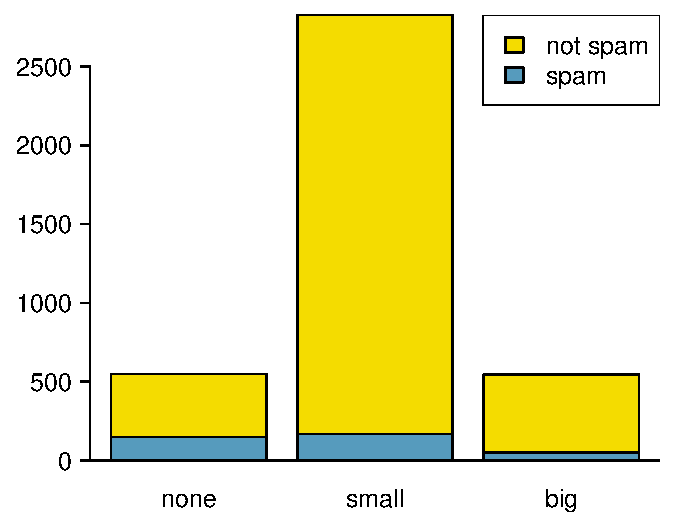
\includegraphics[width=0.46\textwidth]{ch_summarizing_data/figures/emailSpamNumberSegBar/emailSpamNumberSegBar}
\label{emailSpamNumberSegBar}
}
\subfigure[]{
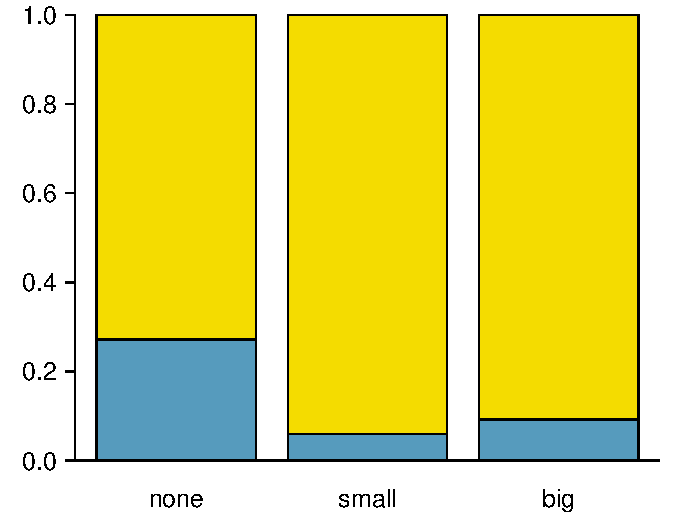
\includegraphics[width=0.46\textwidth]{ch_summarizing_data/figures/emailSpamNumberSegBar/emailSpamNumberSegBarSta}
\label{emailSpamNumberSegBarSta}
}
\caption{\subref{emailSpamNumberSegBar} Segmented bar plot for numbers found in emails, where the counts have been further broken down by \var{spam}. \subref{emailSpamNumberSegBarSta} Standardized version of Figure~\subref{emailSpamNumberSegBar}.}
\label{emailSpamNumberSegBarPlot}
\end{figure}

\begin{example}{Examine both of the segmented bar plots. Which is more useful?}
Figure~\ref{emailSpamNumberSegBar} contains more information, but Figure~\ref{emailSpamNumberSegBarSta} presents the information more clearly. This second plot makes it clear that emails with no number have a relatively high rate of spam email -- about 27\%! On the other hand, less than 10\% of email with small or big numbers are spam.
\end{example}

Since the proportion of spam changes across the groups in Figure~\ref{emailSpamNumberSegBarSta}, we can conclude the variables are dependent, which is something we were also able to discern using table proportions. Because both the \resp{none} and \resp{big} groups have relatively few observations compared to the \resp{small} group, the association is more difficult to see in Figure~\ref{emailSpamNumberSegBar}.

In some other cases, a segmented bar plot that is not standardized will be more useful in communicating important information. Before settling on a particular segmented bar plot, create standardized and non-standardized forms and decide which is more effective at communicating features of the data.


\subsection{The only pie chart you will see in this book}

While pie charts are well known, they are not typically as useful as other charts in a data analysis. A \term{pie chart} is shown in Figure~\ref{emailNumberPieChart} alongside a bar plot. It is generally more difficult to compare group sizes in a pie chart than in a bar plot, especially when categories have nearly identical counts or proportions. In the case of the \resp{none} and \resp{big} categories, the difference is so slight you may be unable to distinguish any difference in group sizes for either~plot!

\begin{figure}
   \centering
   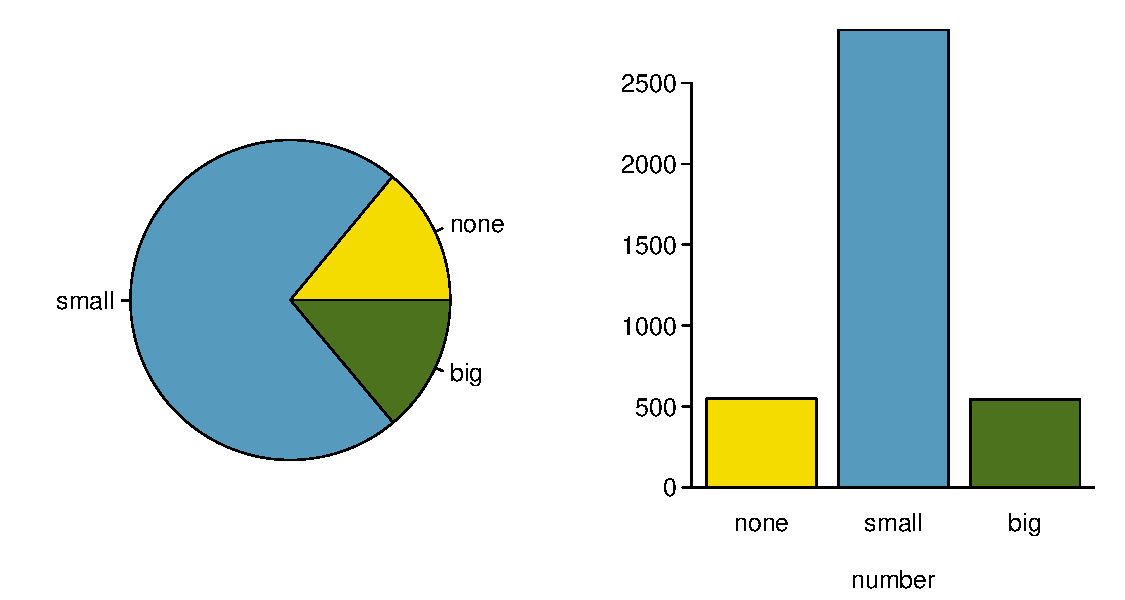
\includegraphics[width=\textwidth]{ch_summarizing_data/figures/emailNumberPieChart/emailNumberPieChart}
   \caption{A pie chart and bar plot of \var{number} for the \data{email} data set.}
   \label{emailNumberPieChart}
\end{figure}

\index{data!email|)}


%___________________________________________
\section{Case study: gender discrimination (special topic)}
\label{caseStudyGenderDiscrimination}

\index{data!discrimination|(}

\begin{example}{Suppose your professor splits the students in class into two groups: students on the left and students on the right. If $\hat{p}_{_L}$ and $\hat{p}_{_R}$ represent the proportion of students who own an Apple product on the left and right, respectively, would you be surprised if $\hat{p}_{_L}$ did not {exactly} equal $\hat{p}_{_R}$?}\label{classRightLeftSideApple}
While the proportions would probably be close to each other, it would be unusual for them to be exactly the same. We would probably observe a small difference due to {chance}.
\end{example}

\begin{exercise}
If we don't think the side of the room a person sits on in class is related to whether the person owns an Apple product, what assumption are we making about the relationship between these two variables?\footnote{We would be assuming that these two variables are independent.}
\end{exercise}

\subsection{Variability within data}
\label{variabilityWithinData}

We consider a study investigating gender discrimination in the 1970s, which is set in the context of personnel decisions within a bank.\footnote{Rosen B and Jerdee T. 1974. Influence of sex role stereotypes on personnel decisions. Journal of Applied Psychology 59(1):9-14.} The research question we hope to answer is, ``Are females unfairly discriminated against in promotion decisions made by male managers?"

The participants in this study are 48 male bank supervisors attending a management institute at the University of North Carolina in 1972. They were asked to assume the role of the personnel director of a bank and were given a personnel file to judge whether the person should be promoted to a branch manager position. The files given to the participants were identical, except that half of them indicated the candidate was male and the other half indicated the candidate was female. These files were randomly assigned to the subjects.

\begin{exercise}
Is this an observational study or an experiment? What implications does the study type have on what can be inferred from the results?\footnote{The study is an experiment, as subjects were randomly assigned a male file or a female file. Since this is an experiment, the results can be used to evaluate a causal relationship between gender of a candidate and the promotion decision.}
\end{exercise}

For each supervisor we record the gender associated with the assigned file and the promotion decision. Using the results of the study summarized in Table~\ref{discriminationResults}, we would like to evaluate if females are unfairly discriminated against in promotion decisions. In this study, a smaller proportion of females are promoted than males (0.583 versus 0.875), but it is unclear whether the difference provides \emph{convincing evidence} that females are unfairly discriminated against.

\begin{table}[ht]
\centering
\begin{tabular}{l l cc rr}
& & \multicolumn{2}{c}{\var{decision}} \\
  \cline{3-4}
		&			& 	{promoted} 	& {not promoted} & Total & \hspace{3mm} \\
  \cline{2-5}
		&	{male} 			& 21    		& 3   & 24  	 \\
  \raisebox{1.5ex}[0pt]{\var{gender}}		&	{female} 	& 14    		& 10     & 24	 \\
  \cline{2-5}
  		&	Total		& 35	& 13	&  48 \\
  \cline{2-5}
\end{tabular}
\caption{Summary results for the gender discrimination study.}
\label{discriminationResults}
\end{table}

\begin{example}{Statisticians are sometimes called upon to evaluate the strength of evidence. When looking at the rates of promotion for males and females in this study, what comes to mind as we try to determine whether the data show convincing evidence of a real difference?} \label{discriminationResultsWhatIsConvincingEvidence}
The observed promotion rates (58.3\% for females versus 87.5\% for males) suggest there might be discrimination against women in promotion decisions. However, we cannot be sure if the observed difference represents discrimination or is just from random chance. Generally there is a little bit of fluctuation in sample data, and we wouldn't expect the sample proportions to be \emph{exactly} equal, even if the truth was that the promotion decisions were independent of gender.
\end{example}

Example~\ref{discriminationResultsWhatIsConvincingEvidence} is a reminder that the observed outcomes in the sample may not perfectly reflect the true relationships between variables in the underlying population. Table~\ref{discriminationResults} shows there were 7 fewer promotions in the female group than in the male group, a difference in promotion rates of 29.2\% $\left( \frac{21}{24} - \frac{14}{24} = 0.292 \right)$. This difference is large, but the sample size for the study is small, making it unclear if this observed difference represents discrimination or whether it is simply due to chance. We label these two competing claims, $H_0$ and $H_A$:
\begin{itemize}
\setlength{\itemsep}{0mm}
\item[$H_0$:] \textbf{Independence model.} The variables \var{gender} and \var{decision} are independent. They have no relationship, and the observed difference between the proportion of males and females who were promoted, 29.2\%, was due to chance.
\item[$H_A$:] \textbf{Alternative model.} The variables \var{gender} and \var{decision} are \emph{not} independent. The difference in promotion rates of 29.2\% was not due to chance, and equally qualified females are less likely to be promoted than males.
\end{itemize}

What would it mean if the independence model, which says the variables \var{gender} and \var{decision} are unrelated, is true? It would mean each banker was going to decide whether to promote the candidate without regard to the gender indicated on the file. That~is, the difference in the promotion percentages was due to the way the files were randomly divided to the bankers, and the randomization just happened to give rise to a relatively large difference of 29.2\%.

Consider the alternative model: bankers were influenced by which gender was listed on the personnel file. If this was true, and especially if this influence was substantial, we would expect to see some difference in the promotion rates of male and female candidates. If this gender bias was against females, we would expect a smaller fraction of promotion decisions for female personnel files relative to the male files.

We choose between these two competing claims by assessing if the data conflict so much with $H_0$ that the independence model cannot be deemed reasonable. If this is the case, and the data support $H_A$, then we will reject the notion of independence and conclude there was discrimination.

\subsection{Simulating the study}
\label{simulatingTheStudy}

Table~\ref{discriminationResults} shows that 35 bank supervisors recommended promotion and 13 did not. Now, suppose the bankers' decisions were independent of gender. Then, if we conducted the experiment again with a different random arrangement of files, differences in promotion rates would be based only on random fluctuation. We can actually perform this \term{randomization}, which simulates what would have happened if the bankers' decisions had been independent of gender but we had distributed the files differently.

In this \term{simulation}, we thoroughly shuffle 48 personnel files, 24 labeled \resp{male\_\hspace{0.3mm}sim} and 24 labeled \resp{female\_\hspace{0.3mm}sim}, and deal these files into two stacks. We will deal 35 files into the first stack, which will represent the 35 supervisors who recommended promotion. The second stack will have 13 files, and it will represent the 13 supervisors who recommended against promotion. Then, as we did with the original data, we tabulate the results and determine the fraction of \resp{male\_\hspace{0.3mm}sim} and \resp{female\_\hspace{0.3mm}sim} who were promoted. The randomization of files in this simulation is independent of the promotion decisions, which means any difference in the two fractions is entirely due to chance. Table~\ref{discriminationRand1} show the results of such a simulation.

\begin{table}[ht]
\centering
\begin{tabular}{l l cc rr}
& & \multicolumn{2}{c}{\var{decision}} \\
  \cline{3-4}
		&			& 	{promoted} 	& {not promoted} & Total & \hspace{3mm} \\
  \cline{2-5}
		&	\resp{male\_\hspace{0.3mm}sim} 					& 18    		& 6    & 24 	 \\
  \raisebox{1.5ex}[0pt]{\var{gender\_\hspace{0.3mm}sim}}		&	\resp{female\_\hspace{0.3mm}sim} 	& 17    		& 7 & 24    	 \\
  \cline{2-5}
  & Total	& 35 & 13 & 48
\end{tabular}
\caption{Simulation results, where any difference in promotion rates between \resp{male\_\hspace{0.3mm}sim} and \resp{female\_\hspace{0.3mm}sim} is purely due to chance.}
\label{discriminationRand1}
\end{table}

\begin{exercise} \label{sampleDifferenceInMaleAndFemaleDiscrimination}
What is the difference in promotion rates between the two simulated groups in Table~\ref{discriminationRand1}? How does this compare to the observed 29.2\% in the actual groups?\footnote{$18/24 - 17/24=0.042$ or about 4.2\% in favor of the men. This difference due to chance is much smaller than the difference observed in the actual groups.}
\end{exercise}


\subsection{Checking for independence}

We computed one possible difference under the independence model in Guided Practice~\ref{sampleDifferenceInMaleAndFemaleDiscrimination}, which represents one difference due to chance. While in this first simulation, we physically dealt out files, it is more efficient to perform this simulation using a computer. Repeating the simulation on a computer, we get another difference due to chance: -0.042. And another: 0.208. And so on until we repeat the simulation enough times that we have a good idea of what represents the \emph{distribution of differences from chance alone}. Figure~\ref{discRandDotPlot} shows a plot of the differences found from 100 simulations, where each dot represents a simulated difference between the proportions of male and female files that were recommended for promotion.

\begin{figure}[ht]
\centering
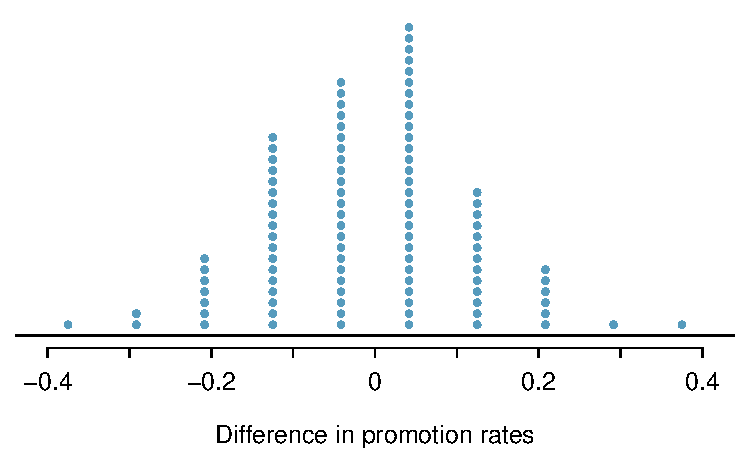
\includegraphics[width=0.7\textwidth]{ch_summarizing_data/figures/discRandDotPlot/discRandDotPlot}
\caption{A stacked dot plot of differences from 100 simulations produced under the independence model, $H_0$, where \var{gender\_\hspace{0.3mm}sim} and \var{decision} are independent. Two of the 100 simulations had a difference of at least 29.2\%, the difference observed in the study.}
\label{discRandDotPlot}
\end{figure}

Note that the distribution of these simulated differences is centered around 0. We simulated these differences assuming that the independence model was true, and under this condition, we expect the difference to be zero with some random fluctuation. We would generally be surprised to see a difference of \emph{exactly} 0: sometimes, just by chance, the difference is higher than 0, and other times it is lower than zero.

\begin{example}{How often would you observe a difference of at least 29.2\% (0.292) according to Figure~\ref{discRandDotPlot}? Often, sometimes, rarely, or never?}
It appears that a difference of at least 29.2\% due to chance alone would only happen about 2\% of the time according to Figure~\ref{discRandDotPlot}. Such a low probability indicates a rare event.
\end{example}

The difference of 29.2\% being a rare event suggests two possible interpretations of the results of the study:
\begin{itemize}
\setlength{\itemsep}{0mm}
\item[$H_0$] \textbf{Independence model.} Gender has no effect on promotion decision, and we observed a difference that would only happen rarely.
\item[$H_A$] \textbf{Alternative model.} Gender has an effect on promotion decision, and what we observed was actually due to equally qualified women being discriminated against in promotion decisions, which explains the large difference of 29.2\%.
\end{itemize}
Based on the simulations, we have two options. (1)~We conclude that the study results do not provide strong evidence against the independence model. That is, we do not have sufficiently strong evidence to conclude there was gender discrimination. (2)~We conclude the evidence is sufficiently strong to reject $H_0$ and assert that there was gender discrimination. When we conduct formal studies, usually we reject the notion that we just happened to observe a rare event.\footnote{This reasoning does not generally extend to anecdotal observations. Each of us observes incredibly rare events every day, events we could not possibly hope to predict. However, in the non-rigorous setting of anecdotal evidence, almost anything may appear to be a rare event, so the idea of looking for rare events in day-to-day activities is treacherous. For example, we might look at the lottery: there was only a 1 in 176 million chance that the Mega Millions numbers for the largest jackpot in history (March 30, 2012) would be (2, 4, 23, 38, 46) with a Mega ball of (23), but nonetheless those numbers came up! However, no matter what numbers had turned up, they would have had the same incredibly rare odds. That is, \emph{any set of numbers we could have observed would ultimately be incredibly rare}. This type of situation is typical of our daily lives: each possible event in itself seems incredibly rare, but if we consider every alternative, those outcomes are also incredibly rare. We should be cautious not to misinterpret such anecdotal evidence.} So in this case, we reject the independence model in favor of the alternative. That is, we are concluding the data provide strong evidence of gender discrimination against women by the supervisors.

\index{data!discrimination|)}

One field of statistics, statistical inference, is built on evaluating whether such differences are due to chance. In statistical inference, statisticians evaluate which model is most reasonable given the data. Errors do occur, just like rare events, and we might choose the wrong model. While we do not always choose correctly, statistical inference gives us tools to control and evaluate how often these errors occur. In Chapter~\ref{foundationsForInference}, we give a formal introduction to the problem of model selection. We spend the next two chapters building a foundation of probability and theory necessary to make that discussion rigorous.